\documentclass[spanish]{thesis}

\addauthor{Xavier R. Verdecie Ramos}
\title{Sistema de carga fragmentada de videos y desacoplamiento del renderizado en Picta}
\ucicenter{Facultad de Tecnologías Interactivas}
\facultynum{4}
\addtutor[Tutor]{MS. C Lisset Salazar Gómez}

\thought{Lo fácil debe ser fácil, lo difí­cil posible\newline Allan Kay}

\dedicatory{
  A mi familia y amigos 

  por ser todo lo que tuve durante estos años tan bonitos.

  A todo aquello que me aportó experiencia, conocimiento y dolores de cabeza.

  A mi gato que nunca dejó de maullar alentadoramente(Creo...).
}

\acknowledgment{
  A mi tutora Lisset, por su guía, paciencia y valiosos aportes durante 
toda mi carrera, no solo durante el desarrollo de mi tesis, sino también
durante los años enseñándome a ser un profesional y llevándome a segundas
convocatorias, merecidamente.

A todos los profesores de la Universidad de las Ciencias Informáticas que me enseñaron realmente, por compartir sus 
conocimientos y contribuir a mi formación profesional durante estos años de estudio.

A la Universidad de las Ciencias Informáticas (UCI) y al Parque Tecnológico de la Habana, especialmente al proyecto Z17, 
por brindarme la oportunidad de trabajar en un proyecto tan grande como este.

A mis compañeros de equipo en Picta, especialmente a Marcos, por su 
colaboración, retroalimentación y por compartir sus experiencias y su tiempo.

A mi familia, por su apoyo incondicional, comprensión y sacrificios realizados para 
que pudiera alcanzar esta meta. Sobre todo a mi madre que jamás dudó ni un segundo en dejarme cumplir mi sueño aunque
estuviese tan lejos de su abrazo, a mi padre, referente eterno en mi vida social, profesional y sentimental, a mi hermano
que fue siempre un apoyo silente pero muy importante desde que empezó este proceso.

A mis amigos, que se convirtieron en un pedacito mas de mi mismo, en una familia nueva, especialmente a 
Bianco, un inesperado hermano a dia de hoy, a Darío, mi compañero intelectual desde el principio, a Beatriz(La Flaca aunque no lo sea), a
Daniela, Osmel, Miguel y a una lista inacabable de personas maravillosas.

A Mary, mi compañera más íntima durante todo este proceso, mi apoyo y consuelo en las noches de soledad, trabajo, estudio, en los momentos mas
duros y los mas felices. Quien se ganó un aprecio eterno e incondicional de mi corazón.

A todos los que de una u otra forma contribuyeron a la realización de este trabajo. Esto no hubiera sido posible sin todos ustedes.

Gracias Totales!
}

\abstract{La insuficiente infraestructura de la red nacional de internet, generadora de bajas velocidades de conexión, impacta negativamente en servicios en línea como la plataforma de streaming Picta. Este contexto afecta específicamente el proceso de subida y renderizado de videos por parte de sus más de 700 canales activos, consumiendo un ancho de banda y recursos del servidor significativos, lo que perjudica la experiencia del usuario y limita la escalabilidad del servicio. La presente investigación se desarrolla con el objetivo de diseñar e implementar un sistema que mitigue estos efectos mediante una estrategia que integra una subida fragmentada de videos y una arquitectura dirigida por eventos para desacoplar la subida del renderizado. La metodología comprendió la caracterización del flujo existente para identificar cuellos de botella, el diseño de la nueva arquitectura y la implementación y evaluación del prototipo. Los principales resultados obtenidos demuestran una mejora sustancial en la experiencia de usuario durante la subida de contenido, otorgándole mayor control, junto con una reducción en el consumo de ancho de banda y una optimización en el uso de los recursos del servidor. Se concluye que la propuesta constituye una solución efectiva para contrarrestar las limitaciones del entorno, garantizando un proceso de publicación más fluido y eficiente, y sentando las bases para una mejor escalabilidad de la plataforma.}

\keywords{arquitectura dirigida por eventos, desacoplamiento de procesos, optimización de recursos de red, plataformas de streaming, subida fragmentada de archivos}

\input{Glossary}
\newacronym{UCI}{UCI}{Universidad de las Ciencias Informáticas}

\newacronymeng{SCADA}{SCADA}{Supervisión, Control y Adquisición de Datos}



\addbibresource{tesis.bib}

\begin{document}
  \SetWatermarkText{}
  \maketitle
  
  \introduction

La infraestructura de telecomunicaciones es un pilar fundamental para el desarrollo y la prestación
de servicios digitales en la era contemporánea. En el contexto nacional \citep{Press2011, Hernandez2021},
la red de Internet presenta insuficiencias en su infraestructura, lo que se traduce de manera tangible
en bajas velocidades de conexión para los usuarios finales. Esta limitación del entorno tecnológico
impacta directamente en la calidad y la eficiencia de los servicios en línea que operan en el país,
generando desafíos técnicos que requieren soluciones innovadoras y adaptadas a estas condiciones
particulares.

Entre estos servicios se encuentra Picta \citep{UCI2025}, la principal plataforma de
streaming nacional, la cual se ve significativamente afectada por esta problemática. Su operación
depende de la capacidad de más de 700 canales activos para subir y publicar su contenido de video de
forma fluida. Sin embargo, los procesos de subida y renderizado de videos, inherentemente intensivos
en el consumo de ancho de banda y recursos computacionales del servidor, se ven severamente
obstaculizados por las limitaciones de la red. Esto se manifiesta en tiempos de carga excesivamente
largos, interrupciones y una alta demanda sostenida sobre los servidores de la plataforma. La
consecuencia directa es una experiencia de usuario deficiente para los creadores de contenido y una
barrera para la escalabilidad y confiabilidad del servicio de Picta, poniendo en riesgo su crecimiento
sostenible.

Partiendo de esta problemática, se formula el \textbf{problema científico}: ¿Cómo contribuir al proceso 
de subida y renderizado de videos en la plataforma Picta para mitigar los efectos de las limitaciones de 
la infraestructura de red nacional, garantizando una experiencia de usuario fluida y uso eficiente de los 
recursos del servidor? Para abordar este problema, se define como \textbf{objeto de estudio} el proceso 
de subida y renderizado de videos, y como \textbf{campo de acción} específico, este mismo proceso dentro 
del ecosistema de la plataforma Picta.

El \textbf{objetivo general} de esta investigación es desarrollar un sistema de subida fragmentada y 
renderizado asíncrono de videos para la plataforma Picta que mejore la eficiencia en el uso de recursos 
y la experiencia del usuario frente a las limitaciones de la infraestructura de red nacional. Para alcanzar 
este propósito, se establecen los siguientes \textbf{objetivos específicos}:

\begin{enumerate}
  \item Caracterizar el flujo actual de subida y renderizado de videos en Picta para identificar
  cuellos de botella y oportunidades de mejora.

  \item Analizar aplicaciones con funcionalidades similares a las requeridas.

  \item Diseñar un sistema de subida fragmentada que permita la persistencia del progreso y el
  control del usuario durante la carga de videos.

  \item Implementar un mecanismo de renderizado asíncrono que separe la subida del video de su
  procesamiento final.

  \item Evaluar el rendimiento del sistema implementado en términos de tiempo de subida, uso de
  ancho de banda y experiencia del usuario.
\end{enumerate}

Para alcanzar los objetivos propuestos, se emplean \textbf{métodos teóricos y empíricos} que 
guían el proceso investigativo. Entre los \textbf{métodos teóricos} se aplican:

\begin{itemize}
  \item \textbf{Análisis-síntesis:} Permite descomponer el proceso de subida y renderizado en 
  sus componentes fundamentales ---transferencia, validación, transcoding--- para identificar 
  cuellos de botella específicos, y posteriormente sintetizar una solución integrada mediante la 
  arquitectura dirigida por eventos.

  \item \textbf{Histórico-lógico:} Posibilita estudiar la trayectoria histórica de los 
  protocolos de transferencia de archivos y sistemas de almacenamiento, extrayendo los principios 
  lógicos fundamentales que se aplican en el diseño de la solución propuesta.

  \item \textbf{Modelación:} Facilita la representación abstracta del sistema mediante diagramas 
  de flujo, patrones arquitectónicos y de diseño, permitiendo estructurar la solución antes de su 
  implementación física.
\end{itemize}

En cuanto a los \textbf{métodos empíricos}, se emplean:

\begin{itemize}
  \item \textbf{Estudio comparativo:} Se realiza un análisis de sistemas homólogos con 
  funcionalidades similares para identificar fortalezas y limitaciones que informan el diseño de 
  la solución especializada para Picta.

  \item \textbf{Observación:} Se aplica para caracterizar el flujo actual de subida y 
  renderizado en la plataforma, identificando patrones de fallo y limitaciones derivadas de la 
  infraestructura de red nacional.

  \item \textbf{Experimentación:} Se ejecutan pruebas de rendimiento del sistema implementado 
  para validar mejoras en tiempo de subida, uso de ancho de banda y experiencia del usuario, 
  comparando métricas antes y después de la intervención.
\end{itemize}

Este documento está organizado en tres capítulos, conclusiones generales y bibliografía. Los
capítulos se estructuran de la siguiente forma:

\begin{enumerate}
  \item \textbf{Capítulo 1: Fundamentación teórica.} Este capítulo realiza un estudio de soluciones
  homólogas, del flujo actual de subida y renderizado de videos en Picta para identificar cuellos de
  botella y oportunidades de mejora. Para este propósito, además se definen herramientas, técnicas,
  tecnologías y metodologías que se emplearán para alcanzar el objetivo general.

  \item \textbf{Capítulo 2: Diseño de la aplicación.} Se realiza el proceso de ingeniería
  correspondiente a la metodología escogida. Se definen los requisitos que debería cumplir el
  programa en la forma de historias de usuario, se presentan los artefactos generados por la
  metodología de desarrollo y se concluye mencionando los patrones arquitectónicos y de diseño que
  sigue la aplicación.

  \item \textbf{Capítulo 3: Implementación y pruebas.} Se definen tareas de ingeniería y se realiza
  el proceso de pruebas de la aplicación. Se finaliza realizando una validación de la solución
  propuesta.
\end{enumerate}

La relevancia científica de esta propuesta radica en la transición hacia un modelo de procesamiento
asíncrono y distribuido, rompiendo con el esquema tradicional de transferencias monolíticas que
penalizan al usuario ante cualquier micro-corte de red. Al emplear una arquitectura dirigida por
eventos, se busca transformar la infraestructura lógica de la plataforma para que sea capaz de
gestionar cargas de trabajo de forma elástica y resiliente \citep{Richards2020}. Este enfoque
permite que el sistema reaccione de manera dinámica ante la disponibilidad de recursos, asegurando
que la etapa de renderización ---crítica por su consumo de CPU--- no comprometa la disponibilidad
inmediata de la interfaz de usuario ni la integridad de los datos en tránsito.

Desde una perspectiva práctica, este trabajo se inserta en el esfuerzo por fortalecer la soberanía
tecnológica y mejorar la accesibilidad de los servicios digitales en el contexto nacional
\citep{Fuentes2025}. Al optimizar el uso de la red mediante la fragmentación de paquetes, se
democratiza la creación de contenido, permitiendo que usuarios con conexiones inestables o de bajo
ancho de banda puedan contribuir de manera efectiva al ecosistema audiovisual de Picta. De este
modo, la solución propuesta trasciende la optimización técnica de un módulo específico para
convertirse en un habilitador de escalabilidad que garantiza la continuidad del servicio frente a
una demanda creciente de tráfico y almacenamiento \citep{Avizienis2004}.

Como \textbf{resultados esperados}, se prevé una mejora tangible en la experiencia de los usuarios
que suben contenido, otorgándoles un mayor control sobre el proceso; una reducción significativa en
el consumo de ancho de banda durante el proceso; y una optimización en la utilización de los recursos
del servidor, lo que en conjunto contribuirá a una mayor robustez y escalabilidad de la plataforma
Picta \citep{Pressman2021}. La presente tesis se organiza para documentar de manera exhaustiva este
proceso, desde el análisis inicial hasta la implementación y validación de la solución propuesta,
con el fin de ofrecer una respuesta técnica viable a un problema de relevancia en el contexto digital
nacional.
  \chapter{Fundamentación Teórica}

El presente capítulo constituye el soporte teórico y técnico sobre el cual se sustenta la propuesta 
de solución para la plataforma Picta. Su propósito es establecer un marco de referencia común que 
permita comprender la complejidad del problema y la validez de la arquitectura propuesta. 

Para ello, la exposición se estructura en cinco momentos fundamentales: primero, se definen los 
conceptos técnicos esenciales que rigen el sistema; segundo, se realiza un estudio comparativo de 
soluciones homólogas en el mercado; tercero, se caracteriza el flujo operativo actual de Picta para 
identificar sus vulnerabilidades; cuarto, se seleccionan las herramientas tecnológicas que integrarán 
la solución; y finalmente, se fundamenta la metodología de desarrollo de software que guiará la 
ejecución del proyecto.

\section{Definiciones y conceptos fundamentales}

Para poder profundizar en el análisis de la infraestructura de Picta, es imprescindible precisar los 
términos técnicos y protocolos que forman la base del sistema objetivo. Esta 
contextualización conceptual garantiza una familiarización con la terminología de 
redes, almacenamiento y procesamiento de video que se empleará de forma recurrente en los capítulos 
posteriores. A continuación, se describen los conceptos clave:

\begin{description}
\sloppy
  \item[Checksum:] El checksum es un valor numérico calculado a partir de una secuencia de datos,
  empleado para verificar la integridad de la información durante su transmisión o almacenamiento.
  Su uso permite detectar alteraciones o corrupciones producidas por fallos de red o de hardware
  \citep{ISO2016}. Es utilizado para validar la integridad
  de cada fragmento de video durante el proceso de subida fragmentada a servicios de almacenamiento de datos.
  Cada trozo recibido debe validarse con su checksum antes de ser almacenado,
  garantizando que no se produjo corrupción de datos durante la transferencia bajo condiciones de
  red inestable.

  \item[Protocolo SSH:] El protocolo SSH (\textit{Secure Shell}) define la arquitectura para el
  inicio de sesión remoto seguro entre computadoras. Provee mecanismos de autenticación robusta y
  protege la integridad y confidencialidad de las comunicaciones mediante cifrado. Constituye el
  sucesor seguro de protocolos como Telnet y métodos de transferencia inseguros como FTP
  \citep{Ylonen2006}.

  \item[Amazon S3:] Amazon Simple Storage Service (Amazon S3) es un servicio de almacenamiento de
  objetos en la nube que ofrece escalabilidad, alta disponibilidad y seguridad para el almacenamiento
  y recuperación de cualquier volumen de datos no estructurados, incluyendo video, imágenes y
  documentos \citep{AWS2023}. Existen sistemas de almacenamiento
  de objetos compatibles con la API de Amazon S3, estos pueden funcionar como servidor de destino para los fragmentos de
  video subidos a una plataforma de streaming. 

  \item[Transcoding:] Proceso de conversión digital entre formatos de codificación de video o audio.
  Comprende la descompresión del contenido original, su transformación ---resolución, tasa de bits,
  códec--- y su recompresión en el formato de destino, con el objetivo de garantizar la
  compatibilidad con distintos dispositivos y condiciones de red \citep{Richardson2003}.
  Esto suele garantizar en muchos sistemas que el procesamiento intensivo de recursos no afecte la 
  interacción del usuario ni obligue a mantener sesiones abiertas innecesariamente.

  \item[Integración \textit{seamless}:] Concepto de arquitectura de software que describe la
  capacidad de un módulo o sistema para integrarse en un entorno existente sin alterar la experiencia
  del usuario ni requerir cambios estructurales en los componentes adyacentes
  \citep{Zhuk2004}. Módulos nuevos, creados con el fin de integrarse con una plataforma en producción sin requerir
  modificaciones significativas en los flujos de autenticación, permisos o gestión de datos existentes, tienen como 
  una buena práctica la integración seamless.

  \item[API:] Una Interfaz de Programación de Aplicaciones (API) define el contrato mediante el
  cual dos componentes de software se comunican. En la arquitectura REST, este contrato se expresa a
  través de recursos, verbos HTTP y representaciones de estado, según los principios establecidos
  en la disertación doctoral de \citet{Fielding2000}. Plataformas como Picta funcionan gracias a estas interfaces
  de programación de aplicaciones, encargándose de manejar la mayor parte de la lógica.

  \item[Frontend y Backend:] En la arquitectura de aplicaciones web, el \textit{frontend} designa
  la capa de presentación con la que interactúa el usuario, mientras que el \textit{backend}
  comprende la lógica de negocio, el acceso a datos y la infraestructura del servidor. Ambas capas
  se comunican mediante interfaces bien definidas \citep{Richards2020}. Muchos sistemas modernos usan estos términos para
  definir una separación clara de responsabilidades entre dos servicios. El frontend reaccionará
  de forma reactiva a los cambios de estado del backend sin necesidad de mantener conexiones persistentes durante el proceso de transcodificación.

  \item[Tarea \textit{ad hoc}:] En gestión de proyectos, una tarea \textit{ad hoc} es una actividad
  no planificada que surge durante la ejecución del proyecto y debe atenderse sin interrumpir el
  flujo principal de trabajo \citep{Wysocki2019}. Durante el proceso de desarrollo usando una metodología ágil, en casi todos los casos con estructura de sprints,
  se permite  la integración controlada de tareas \textit{ad hoc} que surgen de las validaciones con el
  cliente. Estas tareas se incorporan al \textit{Product Backlog} y se priorizan en función de su
  impacto en el objetivo del sprint, sin comprometer la entrega del incremento funcional al cierre de
  la iteración.

  \item[World Wide Web:] Sistema de información distribuida que opera sobre Internet mediante el
  protocolo HTTP, permitiendo la transmisión de documentos de hipertexto e hipermedia. Fue
  concebido originalmente por Tim Berners-Lee en el CERN en 1989
  \citep{BernersLee1992}.

  \item[Framework:] Estructura reutilizable de software que provee un conjunto de abstracciones,
  bibliotecas y convenciones sobre las cuales los desarrolladores construyen aplicaciones. Define
  el esqueleto de la aplicación e invierte el control respecto al código del programador
  \citep{Sommerville2015}.

  \item[SDK:] Un kit de desarrollo de software (\textit{Software Development Kit}) agrupa las
  bibliotecas, herramientas, documentación y ejemplos necesarios para que los desarrolladores
  interactúen programáticamente con una plataforma o servicio determinado
  \citep{Messerschmitt2003}. Un SDK pudiese facilitar operaciones como la creación de buckets, 
  la subida de archivos fragmentados, la validación de checksums y la gestión de metadatos de objetos 
  que se deseen guardar, encapsulando la complejidad de un protocolo y permitiendo que el código del backend 
  se mantenga enfocado en la lógica de negocio.
\end{description}

\section{Sistemas homólogos}

Como parte de la investigación para el desarrollo de la aplicación se realizó un estudio de sistemas
con características similares a las deseadas con el propósito de encontrar una opción que se ajuste a
los requisitos de la tarea o, alternativamente, utilizar el conocimiento obtenido durante el proceso
de investigación en el desarrollo de una solución especializada. 

\begin{description}
\sloppy
  \item[Rsync:] Es una aplicación de línea de comandos que permite la rápida transferencia de
  archivos entre computadoras. Copia las diferencias entre los archivos por lo que en caso de error
  en la transferencia es siempre posible reintentarla con una pérdida mínima de progreso. RSync
  identifica estas diferencias dividiendo los archivos en bloques, generando un checksum para cada
  uno de estos y comparando el resultado. También tiene una función de compresión lo que reduce la
  carga de la red y permite una transferencia más rápida. Finalmente, las transferencias se realizan
  a través del protocolo SSH ofreciendo un alto nivel de seguridad.

  \item[MinIO Client:] MinIO es un sistema de almacenamiento de objetos de alto rendimiento liberado
  bajo la licencia GNU Affero General Public License v3.0. Su API es compatible con el servicio
  Amazon S3 \citep{Gadban2021}. Es capaz de trabajar con información no estructurada como fotos o
  vídeos. MinIO tiene tres componentes: MinIO Server, MinIO Client y MinIO Client SDK. MinIO Client
  es una aplicación de línea de comandos que proporciona una alternativa moderna a comandos UNIX
  como \texttt{ls}, \texttt{cat}, \texttt{cp}, \texttt{mirror} y \texttt{diff}. Soporta sistemas de
  archivos y servicios de almacenamiento en la nube compatibles con Amazon S3
  \citep{Grandhe2026}.

  \item[Filezilla:] Es una aplicación de código abierto liberada bajo la licencia GNU GPL que permite
  interactuar con servidores FTP. Está dividida en Filezilla Client y Filezilla Server, ambos con
  soporte para FTP y FTPS, mientras que el cliente soporta adicionalmente SFTP.
\end{description}

\begin{longtable}[c]{|>{\centering\arraybackslash}p{5cm}|>{\centering\arraybackslash}p{2cm}|>{\centering\arraybackslash}p{2.5cm}|>{\centering\arraybackslash}p{2cm}|}
\caption{Comparación de aplicaciones analizadas}
\label{tb:homologos}\\

\hline
\textbf{Característica} & \textbf{Rsync} & \textbf{MinIO Client} & \textbf{Filezilla} \\
\hline
\endfirsthead

\caption[]{Continuación de la página anterior} \\
\hline
\textbf{Característica} & \textbf{Rsync} & \textbf{MinIO Client} & \textbf{Filezilla} \\
\hline
\endhead

\multicolumn{4}{r}{{Continúa en la próxima página}} \\
\endfoot

\hline
\endlastfoot

Interfaz Gráfica            & No & Sí & Sí \\ \hline
Resistencia a Errores       & Sí & No & No \\ \hline
Filtro de Contenido         & No & No & No \\ \hline
Capacidad de autenticación  & Sí & Sí & Sí \\ \hline

\end{longtable}

Como se aprecia en la Tabla~\ref{tb:homologos}, aunque existen herramientas consolidadas para la
transferencia y gestión de archivos, ninguna ofrece una solución integral que se alinee
completamente con las particularidades del ecosistema de Picta. Herramientas como Rsync destacan
por su robustez y resistencia a fallos de red, pero carecen de una interfaz gráfica orientada a
usuarios no técnicos. Por su parte, opciones como MinIO Client o Filezilla, si bien facilitan la
autenticación y el manejo de objetos, operan como aplicaciones independientes o de línea de
comandos. Esto imposibilita una integración \textit{seamless} dentro del flujo web de la plataforma.

Por consiguiente, el estudio de estos sistemas homólogos permite concluir que la adopción de una
herramienta prefabricada no es viable para este caso de estudio, ya que obligaría a los creadores
de contenido a abandonar el entorno de Picta para utilizar software de terceros, fragmentando la
experiencia de usuario. No obstante, el análisis de sus fortalezas ---como la división en bloques
de Rsync o la compatibilidad S3 de MinIO--- sienta las bases para desarrollar un módulo propio.

\section{Caracterización del flujo actual}

Actualmente, el proceso de publicación en Picta sigue un flujo monolítico y síncrono donde la subida
del video y su posterior renderizado (procesamiento, transcoding y generación de calidades) ocurren de
manera secuencial dentro de una misma transacción. Este esquema presenta tres limitaciones
estructurales que comprometen tanto la experiencia del usuario como la sostenibilidad técnica del
servicio.

En primer lugar, el proceso consume un ancho de banda y recursos del servidor significativos de forma
continua durante toda la operación, dado que cada etapa ---subida, validación, transcoding y
generación de múltiples calidades--- bloquea los recursos hasta su conclusión antes de ceder el
control a la etapa siguiente. En segundo lugar, el flujo es altamente vulnerable a interrupciones de
red: cualquier interrupción durante la transferencia del archivo obliga a reiniciar el proceso
completo desde el inicio, sin posibilidad de reanudación parcial. En tercer lugar, el sistema no
proporciona retroalimentación en tiempo real al usuario sobre el estado de la publicación, lo que
genera incertidumbre e insatisfacción en los creadores de contenido.

El diagrama de la Figura~\ref{fig:flujo_actual} ilustra esta secuencia, destacando los puntos de
fallo y las ineficiencias del modelo actual.

\begin{figure}[H]
  \centering
  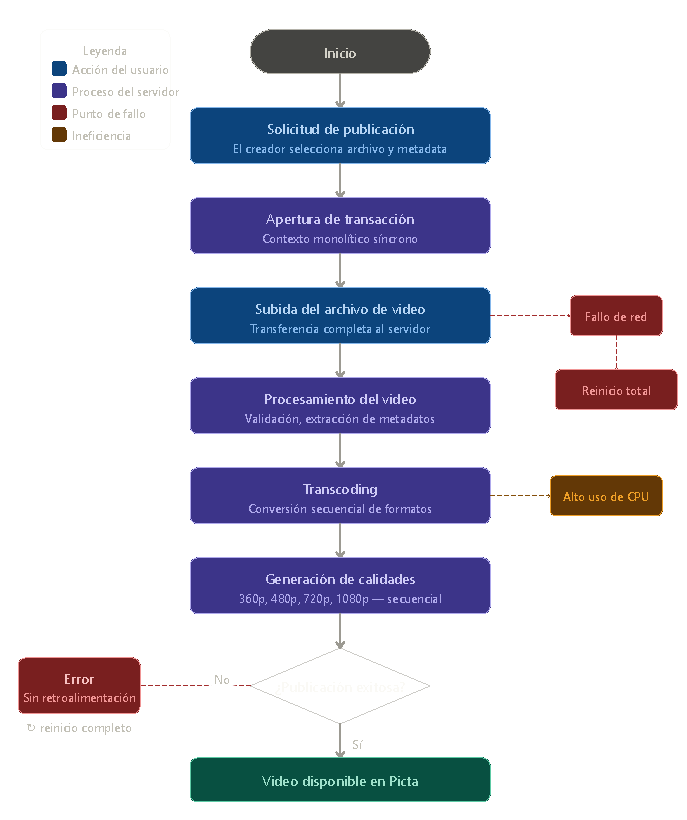
\includegraphics[width=0.9\textwidth]{Images/flujo_actual.pdf}
  \caption{Flujo monolítico y síncrono del proceso de publicación en Picta}
  \label{fig:flujo_actual}
\end{figure}

El conjunto de estas deficiencias genera frustración en los creadores de contenido, ineficiencia en
el uso de los recursos del servidor y limita la escalabilidad horizontal del servicio. Con una
integración transparente en la interfaz existente de Picta, el sistema propuesto será utilizado
tanto por los creadores de contenido como por los administradores de la plataforma, mejorando
radicalmente la resiliencia del servicio ---entendida como la capacidad del sistema de garantizar
la continuidad del proceso ante fallos externos \citep{Avizienis2004}---, la satisfacción del
usuario y la capacidad de la plataforma para crecer de forma sostenible.

\section{Herramientas y Tecnologías}

La selección de las herramientas y tecnologías que integran la solución propuesta responde a un 
criterio de compatibilidad arquitectónica con la plataforma Picta existente, priorizando la cohesión 
del ecosistema tecnológico sobre la adopción de alternativas externas. A continuación, se describen 
el lenguaje de programación, las herramientas de desarrollo y las bibliotecas y \textit{frameworks} 
seleccionados, justificando en cada caso su pertinencia para los objetivos del proyecto.

\subsection{Selección del lenguaje de programación}

La selección del lenguaje para el nuevo módulo está condicionada por la integración con la plataforma
existente. Si bien soluciones alternativas desarrolladas en lenguajes como Golang ofrecerían ventajas
significativas en rendimiento y manejo de concurrencia, la decisión se ve constreñida por la
arquitectura actual del sistema, la cual implementa la API en Python y el frontend en JavaScript,
estableciendo dependencias técnicas que priorizan la cohesión de la plataforma sobre optimizaciones
puntuales.

La evaluación técnica conduce hacia la selección de \textbf{Python} como lenguaje backend. Python
es un lenguaje de programación interpretado, de alto nivel y propósito general, caracterizado por
una sintaxis clara que favorece la legibilidad y reduce el costo de mantenimiento del código.
Cuenta con un amplio ecosistema de bibliotecas para desarrollo web, computación científica y
automatización \citep{Pressman2021}, lo que lo hace especialmente adecuado para la construcción
de módulos de integración como el que se propone.

Paralelamente, para el frontend se mantiene la coherencia arquitectónica mediante la adopción de
\textbf{JavaScript}. Según el estándar ECMAScript, JavaScript es el lenguaje de scripting del lado
del cliente predominante en la Web, y su especificación define el modelo de ejecución, los tipos
de datos y los mecanismos de concurrencia basados en eventos que se utilizarán en el componente
Angular del módulo \citep{Ecma2023}.

\subsection{Herramientas utilizadas}

Las siguientes herramientas fueron empleadas directamente durante el ciclo de desarrollo del módulo,
cubriendo las etapas de codificación, gestión de base de datos, prueba de interfaces y modelado.

\begin{description}
\sloppy
  \item[Visual Studio Code v1.106.2:] Editor de código fuente desarrollado por Microsoft para
  Windows, Linux, macOS y Web. Incluye soporte para depuración, control integrado de Git, resaltado
  de sintaxis, finalización inteligente de código y refactorización. Es software gratuito y de
  código abierto. Fue utilizado como entorno principal de desarrollo del módulo.

  \item[Navicat Premium v17.1.10:] Software de gestión y administración de bases de datos que
  permite conectarse y administrar múltiples motores, incluyendo PostgreSQL, MySQL, MariaDB y
  SQL Server \citep{Sommerville2015}. Se empleó para inspeccionar, consultar y verificar el estado
  de la base de datos de Picta durante el desarrollo e integración del módulo.

  \item[Postman v11.73.3:] Herramienta para el desarrollo, prueba y documentación de APIs. Su
  interfaz gráfica permite construir, enviar y validar solicitudes HTTP de forma sistemática,
  facilitando la verificación de contratos de interfaz \citep{Lutz2013}. Se utilizó para probar
  todos los endpoints de la API desarrollada y documentar el comportamiento del módulo de subida.

  \item[S3 Browser v12.9.9:] Cliente de escritorio para la administración de almacenamiento de
  objetos compatible con el protocolo S3 \citep{AWS2023}. Durante las pruebas, se empleó para
  inspeccionar y verificar la integridad y ubicación de los fragmentos almacenados en el servidor
  MinIO.

  \item[Visual Paradigm v17.0:] Herramienta de modelado visual que implementa el estándar UML 2.0
  \citep{Miles2006}. Se utilizó para la elaboración de los diagramas de casos de uso, clases y
  secuencia del proyecto.
\end{description}

\subsection{Bibliotecas y Frameworks utilizados}

En alineación con los criterios derivados del análisis arquitectónico del sistema vigente y con el
objetivo de garantizar una integración totalmente compatible y sin impactos estructurales, se ha
determinado la adopción de los mismos frameworks actualmente utilizados por la plataforma en sus
componentes principales.

\begin{description}
\sloppy
  \item[Django v3.2.2:] Framework web de alto nivel para Python que implementa el patrón
  Modelo-Vista-Template (MVT) y provee componentes integrados para autenticación, ORM, enrutamiento
  y administración. Fomenta el desarrollo rápido y un diseño limpio bajo el principio
  \textit{Don't Repeat Yourself} (DRY) \citep{Christie2024}.

  \item[Angular v15.2.10:] Framework de desarrollo de aplicaciones web de una sola página (SPA)
  basado en TypeScript, mantenido por Google. Implementa una arquitectura de componentes, inyección
  de dependencias y un sistema de módulos que facilita la escalabilidad del frontend
  \citep{Richards2020}.
\end{description}

Con el fin de garantizar una interacción óptima con MinIO, reducir la complejidad operacional y
estandarizar el flujo de integración, se seleccionaron las siguientes librerías especializadas como
componentes primarios de interoperabilidad.

\begin{description}
\sloppy
  \item[Django Rest Framework v3.12.4:] Conjunto de herramientas para la construcción de APIs web
  sobre Django. Provee serializadores, vistas basadas en clases, autenticación y negociación de
  contenido, simplificando la creación de interfaces RESTful robustas y escalables
  \citep{Christie2024}.

  \item[MinIO Python SDK v7.2.18:] SDK de cliente Python que provee una API de alto nivel para
  interactuar con servidores MinIO y cualquier almacenamiento compatible con el protocolo Amazon S3.
  Gestiona operaciones de carga, descarga, listado y eliminación de objetos \citep{MinIO2024}.
\end{description}

\section{Selección de una metodología de desarrollo}

Una metodología de desarrollo de software es un conjunto de prácticas, técnicas y herramientas
utilizadas por los equipos de desarrollo de software para planificar, diseñar, construir, probar y
entregar software de alta calidad de manera eficiente y efectiva \citep{Pressman2021}.

Las metodologías de desarrollo se dividen actualmente en dos enfoques generales: el tradicional y
el ágil. Las metodologías tradicionales se caracterizan por fases predefinidas con un flujo del
desarrollo unidireccional, pasando de la recolección de requisitos al diseño y del diseño al
desarrollo, luego a las pruebas y el mantenimiento. En aproximaciones clásicas como el modelo de
cascada, cada fase genera artefactos y documentación que han pasado por un extensivo proceso de
revisión \citep{Sommerville2015}. Los métodos tradicionales son mejor utilizados en situaciones en
las que los requisitos están bien definidos. En industrias que cambian rápidamente, como la del
desarrollo de software, las metodologías tradicionales pueden fallar en alcanzar sus objetivos.

Dado que los requisitos del módulo a desarrollar son evolutivos ---determinados por la integración
progresiva con una plataforma en producción--- se descarta el enfoque tradicional y se orienta la
selección hacia las metodologías ágiles. Dentro de este grupo, los marcos de trabajo más relevantes
para proyectos de desarrollo de software de alcance acotado son Scrum, Kanban y Extreme Programming
(XP), cuyas características se comparan en la Tabla~\ref{tb:metodologias_agiles}.

\begin{longtable}[c]{|p{2.3cm}|p{5.5cm}|p{5.3cm}|}
\caption{Comparativa de metodologías ágiles}
\label{tb:metodologias_agiles}\\
\hline
\textbf{Metodología} & \textbf{Ventajas} & \textbf{Desventajas} \\
\hline
\endfirsthead
\caption[]{Continuación de la página anterior} \\
\hline
\textbf{Metodología} & \textbf{Ventajas} & \textbf{Desventajas} \\
\hline
\endhead
\multicolumn{3}{r}{{Continúa en la próxima página}} \\
\endfoot
\hline
\endlastfoot

Scrum &
Iteraciones cortas y planificadas (\textit{sprints}). Roles bien definidos. Revisión continua con
el cliente. Adecuado para equipos pequeños y proyectos de complejidad media-alta
\citep{Schwaber2020}. &
Requiere disponibilidad regular del cliente. Puede generar sobrecarga de reuniones si no se
gestiona. Difícil de escalar sin adaptaciones. \\ \hline

Kanban &
Flujo continuo sin iteraciones fijas. Bajo costo de adopción. Útil para equipos con carga variable
o trabajo de mantenimiento \citep{Pressman2021}. &
Sin estructura de planificación temporal. Dificulta la estimación de plazos. Poco adecuado para
proyectos con entregas definidas y cliente activo. \\ \hline

Extreme Programming (XP) &
Énfasis en calidad técnica: pruebas continuas, integración frecuente, refactorización constante.
Adecuado cuando la calidad del código es prioritaria \citep{Pressman2021}. &
Requiere un equipo de al menos dos desarrolladores para prácticas como la programación en pares.
Alta disciplina técnica exigida desde el inicio. \\ \hline

\end{longtable}

Del análisis comparativo se desprende que \textbf{Kanban} no resulta adecuado para este proyecto,
dado que no provee una estructura de planificación temporal que permita gestionar entregas acordadas
con el tutor y el cliente. \textbf{XP}, por su parte, presupone un equipo mínimo de dos
desarrolladores para aplicar sus prácticas centrales ---como la programación en pares y las pruebas
de aceptación en cliente--- lo que lo hace inviable en el contexto de un desarrollador único. En
consecuencia, se selecciona \textbf{SCRUM} como metodología de desarrollo.

Scrum es un marco de trabajo para el desarrollo ágil de software, cuya guía definitiva fue
publicada por sus cocreadores Ken Schwaber y Jeff Sutherland \citep{Schwaber2020}. Es un proceso
en el que se aplican de manera regular un conjunto de buenas prácticas para trabajar
colaborativamente, en equipo y obtener el mejor resultado posible de proyectos, caracterizado por:

\begin{itemize}
  \item Adoptar una estrategia de desarrollo incremental, en lugar de la planificación y ejecución
  completa del producto.

  \item Basar la calidad del resultado más en el conocimiento tácito de las personas en equipos
  autoorganizados, que en la calidad de los procesos empleados.

  \item Solapar las diferentes fases del desarrollo, en lugar de realizar una tras otra en un ciclo
  secuencial o en cascada.
\end{itemize}

Scrum es un marco de trabajo que resulta fácil de aprender, pero difícil de dominar. La esencia
de \textit{Scrum} es un equipo autoorganizado que aporta valor al cliente en períodos limitados
conocidos como \textit{Sprints} \citep{Sutherland2014}.

\begin{figure}[H]
  \centering
  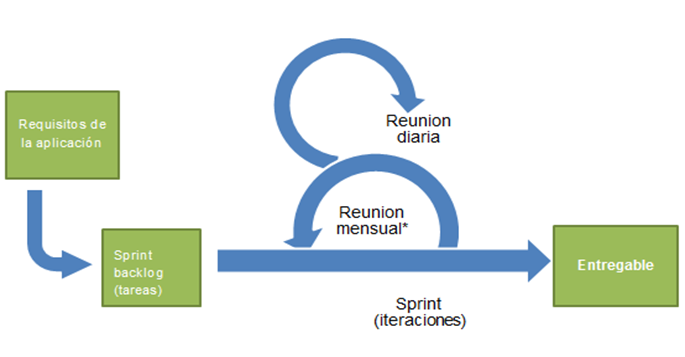
\includegraphics[width=0.9\textwidth]{Images/scrum}
  \caption{Marco de Trabajo SCRUM. Fuente: Adaptado de \citep{AnaDianaMets2013}}
  \label{fig:scrum}
\end{figure}

\subsection{Roles en SCRUM}

La estructura de Scrum se articula en torno a tres roles fundamentales, cada uno con
responsabilidades claramente delimitadas que garantizan el funcionamiento del marco de trabajo
\citep{Schwaber2020}.

El \textbf{Product Owner} es el responsable de maximizar el valor del producto. Representa los
intereses del cliente y de los usuarios finales, gestiona y prioriza el \textit{Product Backlog}
---la lista ordenada de todo lo que el producto podría necesitar--- y toma las decisiones finales
sobre qué se construye y en qué orden. Su efectividad depende directamente de su disponibilidad y
conocimiento del dominio del problema.

El \textbf{Scrum Master} es el garante del proceso \citep{Avizienis2004}. Su función no es la de
un jefe de proyecto tradicional, sino la de un facilitador que protege al equipo de impedimentos
externos, vela por la correcta aplicación del marco Scrum, y promueve la mejora continua a través
de las retrospectivas de sprint. En equipos pequeños, el Scrum Master asume además una función de
\textit{coaching} técnico, orientando las decisiones de diseño y arquitectura cuando el equipo
carece de experiencia suficiente.

El \textbf{Equipo de Desarrollo} está compuesto por los profesionales que ejecutan el trabajo de
construcción del producto. Scrum no prescribe roles internos dentro del equipo ---no hay
distinción formal entre frontend, backend o QA--- y en su lugar promueve la autoorganización: el
equipo decide colectivamente cómo abordar cada ítem del sprint para alcanzar el objetivo acordado
\citep{Cohn2004}.

En el contexto particular de este proyecto, la reducción del equipo a un único integrante implica
la fusión de los roles de \textbf{Scrum Master} y \textbf{Equipo de Desarrollo} en una misma
persona. Esta configuración es viable siempre que el rol de Product Owner permanezca diferenciado
y sea asumido por el cliente \citep{Pierra2022}. En este caso, dicho rol corresponde al
representante de la plataforma Picta, quien valida los incrementos al cierre de cada sprint y
prioriza el backlog en función de las necesidades operativas de la plataforma. El desarrollador
asume el rol de Scrum Master porque es quien posee el conocimiento más profundo de la arquitectura
propuesta, la capacidad para identificar impedimentos técnicos de forma temprana y la
responsabilidad directa de garantizar que cada sprint produzca un incremento funcional e integrable
sobre la plataforma en producción.

La elección de SCRUM para este proyecto se fundamenta en tres factores determinantes que se alinean
con sus fortalezas estructurales. En primer lugar, el equipo de desarrollo está integrado por un
único desarrollador, lo que hace que la ligereza organizativa de Scrum ---frente a metodologías
más pesadas--- sea una ventaja directa. En segundo lugar, el cliente de la plataforma Picta dispone
de alta disponibilidad técnica y conocimiento del dominio, lo que facilita la validación de los
incrementos al cierre de cada sprint. En tercer lugar, la complejidad del proyecto ---integración
de subida fragmentada con arquitectura dirigida por eventos sobre una plataforma en producción---
se ubica dentro del rango de complejidad media-alta que Scrum gestiona con mayor eficacia que un
flujo continuo como Kanban \citep{Schwaber2020}.

\section{Conclusiones Parciales}

El análisis del flujo actual de publicación en Picta evidenció tres limitaciones estructurales ---
consumo continuo de recursos, vulnerabilidad ante interrupciones de red y ausencia de
retroalimentación en tiempo real--- que justifican el desarrollo de una solución especializada. El
estudio de sistemas homólogos confirmó que ninguna herramienta existente satisface los requisitos
de integración \textit{seamless} propios del ecosistema de la plataforma, sentando las bases para
un módulo propio. En este capítulo se definieron además los lenguajes de programación, herramientas,
\textit{frameworks}, librerías y la metodología SCRUM como marco de desarrollo, sustentados en
fuentes primarias y estándares internacionales de la disciplina.
  \chapter{Propuesta de Solución}

El diagnóstico de las limitaciones actuales en la gestión de medios de la plataforma Picta establece el punto 
de partida para la concepción de una solución técnica integral. La transición hacia una arquitectura dirigida 
por eventos demanda la formalización de especificaciones y el modelado de requisitos mediante historias de usuario, 
permitiendo traducir las necesidades detectadas en funcionalidades concretas. Asimismo, la estructuración de un plan 
de entrega sustentado en estimaciones de esfuerzo objetivas, en conjunto con la selección estratégica de patrones arquitectónicos, 
garantiza que la propuesta sea no solo viable desde el punto de vista técnico, sino también plenamente integrable y escalable dentro 
del ecosistema tecnológico existente.

\section{Propuesta de solución}

Teniendo en cuenta que la necesidad de darle solución a las deficiencias de la plataforma es
inminente, este documento propone el desarrollo de un módulo que deberá integrarse al sistema que
actualmente se encuentra funcionando en producción. El módulo tendrá como objetivo ofrecer el servicio
de subida de multimedia a los servidores de Picta con una resistencia a errores que permita recuperar
el progreso de la subida en caso de cualquier situación inesperada, mientras mantiene el uso del
servicio limitado a las personas con los permisos necesarios para administrar un canal. Además,
mediante el desacoplamiento de la subida y el renderizado de videos, se logrará una alta reducción de
carga de trabajo del lado del cliente. Más formalmente se desea que la integración del módulo permita:

\begin{itemize}
  \item \textbf{Gestionar la lista de subida de videos:} El módulo debe brindar a la web la
  posibilidad de manipular los estados de cada subida de video por parte de un administrador de canal,
  dándole opciones de cambiar su estado a `en curso', `pausada', `cancelada' y mantener una
  persistencia de estos datos en el servidor a largo plazo.

  \item \textbf{Pausar subidas de forma arbitraria:} La web debe ser capaz gracias a las
  funcionalidades brindadas por el módulo de cambiar arbitrariamente al estado `pausada' cualquier
  subida que se encuentre `en curso'.

  \item \textbf{Reanudar subidas con estado `pausada':} Luego de cambiar el estado a `pausada', el
  módulo web debe permitirle al cliente autorizado reanudar el proceso desde el punto en que estaba
  antes de cambiar a ese estado, ya sea de forma automática al haber perdido comunicación con el
  servidor o manual al haber elegido arbitrariamente detener momentáneamente el proceso.

  \item \textbf{Persistir históricamente registros de subidas en estado `cancelada':} La web debe ser
  capaz de mostrarle al cliente autorizado todas las subidas con estado `cancelada' que haya
  registrado.

  \item \textbf{Procesar arbitrariamente metadatos de videos subidos al servidor S3:} El módulo web
  debe permitirle al usuario autorizado, luego de haber terminado la subida de un video al servidor
  S3, procesar del lado de la API los metadatos relacionados con el video en cuestión.

  \item \textbf{Listar videos sin metadatos aún asociados:} El sistema debe, gracias al módulo web,
  mostrarle al usuario autorizado una lista de videos ya subidos al servidor de MinIO S3 pero que aún
  no han sido renderizados con los metadatos necesarios.
\end{itemize}

\section{Posibles estados de una subida}

A continuación, se describe un diagrama de flujo orientado a los posibles estados que deberá poder
tomar una subida de videos según el nuevo módulo web:

\begin{figure}[htbp]
  \centering
  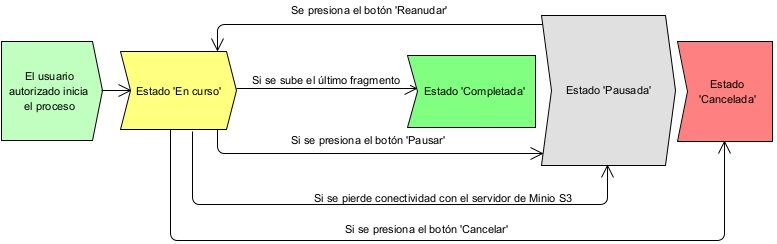
\includegraphics[width=0.95\textwidth]{Images/flujo_estados}
  \caption{Flujo de posibles estados de una subida. Elaboración propia}
  \label{fig:flujo_estados}
\end{figure}

A continuación, se describe un diagrama de flujo orientado a ilustrar la lógica que deberá tomar un
proceso de subida de videos según el nuevo módulo web:

\begin{figure}[htbp]
  \centering
  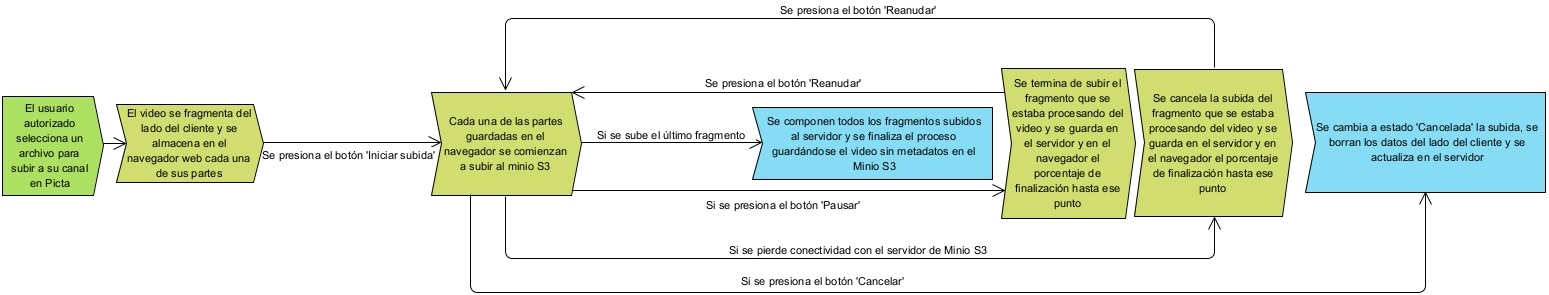
\includegraphics[width=0.95\textwidth]{Images/flujo_proceso}
  \caption{Flujo del proceso de subida de videos. Elaboración propia}
  \label{fig:flujo_proceso}
\end{figure}
 
\section{Historias de Usuario}

De acuerdo con \citep{Cohn2004}, las historias de usuario son uno de los principales
artefactos de desarrollo para los equipos de Scrum y Programación Extrema (XP). Una historia de
usuario es una definición de alto nivel de un requisito, que contiene la información justa para que
los desarrolladores puedan estimar razonablemente el esfuerzo necesario para implementarlo.

Como parte de la metodología Scrum se realizaron varias historias de usuario con el objetivo de tener
una mejor comprensión de los requisitos de la aplicación. A continuación, se presentan las historias
generadas.

\newcommand{\huhead}[4]{%
  \multicolumn{2}{|l|}{\colorentry{\textbf{Historia de Usuario}}} \\
  \hline
  \textbf{Número:} #1 \quad \textbf{Estimación:} #2 & \textbf{Sprint:} #3 \\
  \hline
  \multicolumn{2}{|p{13.5cm}|}{\textbf{Nombre:} #4} \\
  \hline
}

\newcommand{\huestereotipo}[3]{%
  % #1 = ruta de imagen, #2 = label, #3 = texto del caption
  \multicolumn{2}{|l|}{\textbf{Prototipo:}} \\
  \hline
  \multicolumn{2}{|p{13.5cm}|}{%
    \vspace{4pt}%
    \centering
    \includegraphics[width=0.75\linewidth]{#1}%
    \refstepcounter{figure}%
    \addcontentsline{lof}{figure}{\protect\numberline{\thefigure}#3}%
    \label{#2}%
    \par\smallskip
    {\small \textbf{Figura~\thefigure:} #3}%
    \vspace{4pt}%
  } \\
  \hline
}

% ── HU-01 ─────────────────────────────────────────────────────────────────────
\begin{longtable}[c]{|p{3.5cm}|p{10cm}|}
\caption{HU-01 Crear publicación y abrir popup de subida}
\label{tb:hu01}\\
\hline
\huhead{HU-01}{8 h}{1}{Crear publicación y abrir popup de subida}
\textbf{Prioridad de Negocio:} Crítica & \textbf{Asignado a:} Xavier Verdecie \\
\hline
\multicolumn{2}{|l|}{\textbf{Descripción:}} \\
\hline
\multicolumn{2}{|p{13.5cm}|}{Como administrador de canal de Picta, quiero poder crear una
publicación definiendo sus metadatos básicos (título, canal, categoría) y al guardar que se abra un
popup con una barra de progreso en 0\% con opciones para iniciar o cancelar la subida, para tener
control explícito sobre cuándo comienza la transferencia del archivo.} \\
\hline
\multicolumn{2}{|l|}{\textbf{Criterio de Aceptación:}} \\
\hline
\multicolumn{2}{|p{13.5cm}|}{\textbf{Given (Dado que):} El administrador de canal está autenticado y
accede al formulario de creación de publicación.} \\
\hline
\multicolumn{2}{|p{13.5cm}|}{\textbf{When (Cuando):} Completa los campos obligatorios (título, canal,
categoría, archivo de video) y presiona `Guardar'.} \\
\hline
\multicolumn{2}{|p{13.5cm}|}{\textbf{Then (Entonces):} Se registra la publicación en estado
`pendiente' y se muestra un popup modal con: barra de progreso en 0\%, botones `Iniciar' y
`Cancelar', y una cruz (X) arriba a la izquierda para cerrar y navegar a la página de gestión de
subidas.} \\
\hline
\multicolumn{2}{|l|}{\textbf{Validaciones:}} \\
\hline
\multicolumn{2}{|p{13.5cm}|}{\textbf{Frontend:} Validar campos obligatorios antes de permitir guardar.
Llamar a endpoint especializado para validar datos. El popup debe ser modal (bloquear interacción con
el fondo).\newline
\textbf{Backend:} Verificar token de sesión y permisos de administrador de canal antes de registrar la
publicación. Validar datos correctamente cuando se acceda al endpoint especializado.} \\
\hline
\multicolumn{2}{|l|}{\textbf{Observaciones:}} \\
\hline
\multicolumn{2}{|p{13.5cm}|}{Esta HU separa la creación de metadatos del inicio de la subida,
permitiendo al usuario revisar antes de comenzar la transferencia. La cruz del popup redirige
directamente a la página de gestión para facilitar el seguimiento de múltiples subidas.} \\
\hline
\huestereotipo{Images/Iniciar - Initial.jpg}{fig:hu01_estereotipo}{Prototipo de la HU-01:
  Interfaz del popup inicial de subida con barra de progreso en 0\% y botones Iniciar/Cancelar.
  Elaborado con Visual Paradigm como referencia visual.}
\end{longtable}

% ── HU-02 ─────────────────────────────────────────────────────────────────────
\begin{longtable}[c]{|p{3.5cm}|p{10cm}|}
\caption{HU-02 Iniciar proceso de carga fragmentada}
\label{tb:hu02}\\
\hline
\huhead{HU-02}{18 h}{1}{Iniciar proceso de carga fragmentada}
\textbf{Prioridad de Negocio:} Crítica & \textbf{Asignado a:} Xavier Verdecie \\
\hline
\multicolumn{2}{|l|}{\textbf{Descripción:}} \\
\hline
\multicolumn{2}{|p{13.5cm}|}{Como administrador de canal, quiero que al presionar `Iniciar' en el
popup de subida, el sistema divida el archivo en fragmentos y comience la transferencia de forma
controlada y tolerante a fallos de red, mostrando el progreso en tiempo real.} \\
\hline
\multicolumn{2}{|l|}{\textbf{Criterio de Aceptación:}} \\
\hline
\multicolumn{2}{|p{13.5cm}|}{\textbf{Given (Dado que):} El popup de subida está abierto con progreso
en 0\%.} \\
\hline
\multicolumn{2}{|p{13.5cm}|}{\textbf{When (Cuando):} El usuario presiona el botón `Iniciar'.} \\
\hline
\multicolumn{2}{|p{13.5cm}|}{\textbf{Then (Entonces):} El sistema registra una nueva sesión de subida
con estado `en curso', divide el archivo en fragmentos de tamaño configurable, calcula el checksum de
cada fragmento, comienza la transferencia secuencial al servidor MinIO S3, actualiza la barra de
progreso en tiempo real, y cambia los botones disponibles a `Pausar' y `Cancelar'.} \\
\hline
\multicolumn{2}{|l|}{\textbf{Validaciones:}} \\
\hline
\multicolumn{2}{|p{13.5cm}|}{\textbf{Frontend:} Deshabilitar el botón `Iniciar' una vez presionado.
Mostrar progreso por fragmento y global. Manejar errores de red con reintentos automáticos.\newline
\textbf{Backend:} Validar token de sesión. Cada fragmento recibido debe validarse con su checksum
(MD5/SHA256) \citep{Stallings2017} antes de almacenarse en MinIO. Rechazar solicitudes de roles sin
permisos.} \\
\hline
\multicolumn{2}{|l|}{\textbf{Observaciones:}} \\
\hline
\multicolumn{2}{|p{13.5cm}|}{Esta HU implementa el núcleo del protocolo de carga fragmentada sobre
Django REST Framework, utilizando minio-py v7.2.18. La lógica de partición reside en Angular v15.} \\
\hline
\huestereotipo{Images/Iniciar - Initial.jpg}{fig:hu02_estereotipo}{Prototipo de la HU-02:
  Popup de subida en curso mostrando progreso en tiempo real y botones Pausar/Cancelar.
  Elaborado con Visual Paradigm como referencia visual.}
\end{longtable}

% ── HU-03 ─────────────────────────────────────────────────────────────────────
\begin{longtable}[c]{|p{3.5cm}|p{10cm}|}
\caption{HU-03 Pausar subida de video en curso}
\label{tb:hu03}\\
\hline
\huhead{HU-03}{10 h}{1}{Pausar subida de video en curso}
\textbf{Prioridad de Negocio:} Alta & \textbf{Asignado a:} Xavier Verdecie \\
\hline
\multicolumn{2}{|l|}{\textbf{Descripción:}} \\
\hline
\multicolumn{2}{|p{13.5cm}|}{Como administrador de canal, quiero poder pausar una subida en curso
presionando el botón `Pausar' en el popup, para interrumpir temporalmente la transferencia sin perder
el progreso.} \\
\hline
\multicolumn{2}{|l|}{\textbf{Criterio de Aceptación:}} \\
\hline
\multicolumn{2}{|p{13.5cm}|}{\textbf{Given (Dado que):} Una subida está en curso con estado `en
curso'.} \\
\hline
\multicolumn{2}{|p{13.5cm}|}{\textbf{When (Cuando):} El usuario presiona `Pausar' en el popup.} \\
\hline
\multicolumn{2}{|p{13.5cm}|}{\textbf{Then (Entonces):} El frontend detiene el envío de nuevos
fragmentos, persiste el número del último fragmento enviado exitosamente, cambia el estado de la
sesión a `pausada', y actualiza los botones disponibles a `Reanudar' y `Cancelar'.} \\
\hline
\multicolumn{2}{|l|}{\textbf{Validaciones:}} \\
\hline
\multicolumn{2}{|p{13.5cm}|}{\textbf{Frontend:} Esperar confirmación del último fragmento en tránsito
antes de pausar. No permitir pausar si estado no es `en curso'. Si el navegador se cierra por algún
motivo o hay un timeout el proceso debe también cambiar al estado `pausada'.\newline
\textbf{Backend:} Validar que el usuario sea el propietario de la sesión.} \\
\hline
\multicolumn{2}{|l|}{\textbf{Observaciones:}} \\
\hline
\multicolumn{2}{|p{13.5cm}|}{La pausa arbitraria permite optimizar el uso del ancho de banda en
horarios de alto tráfico o liberar recursos temporalmente.} \\
\hline
\huestereotipo{Images/Pausar - Initial.jpg}{fig:hu03_estereotipo}{Prototipo de la HU-03:
  Popup con subida pausada mostrando botones Reanudar/Cancelar.
  Elaborado con Visual Paradigm como referencia visual.}
\end{longtable}

% ── HU-04 ─────────────────────────────────────────────────────────────────────
\begin{longtable}[c]{|p{3.5cm}|p{10cm}|}
\caption{HU-04 Reanudar subida pausada}
\label{tb:hu04}\\
\hline
\huhead{HU-04}{12 h}{1}{Reanudar subida pausada}
\textbf{Prioridad de Negocio:} Alta & \textbf{Asignado a:} Xavier Verdecie \\
\hline
\multicolumn{2}{|l|}{\textbf{Descripción:}} \\
\hline
\multicolumn{2}{|p{13.5cm}|}{Como administrador de canal, quiero poder reanudar una subida pausada
presionando el botón `Reanudar' en el popup, para continuar la transferencia desde el último fragmento
enviado exitosamente.} \\
\hline
\multicolumn{2}{|l|}{\textbf{Criterio de Aceptación:}} \\
\hline
\multicolumn{2}{|p{13.5cm}|}{\textbf{Given (Dado que):} Una subida está en estado `pausada'.} \\
\hline
\multicolumn{2}{|p{13.5cm}|}{\textbf{When (Cuando):} El usuario presiona `Reanudar' en el popup.} \\
\hline
\multicolumn{2}{|p{13.5cm}|}{\textbf{Then (Entonces):} El frontend consulta el último fragmento
registrado en el backend, reanuda la transferencia desde el siguiente fragmento, actualiza el estado a
`en curso', y cambia los botones disponibles a `Pausar' y `Cancelar'.} \\
\hline
\multicolumn{2}{|l|}{\textbf{Validaciones:}} \\
\hline
\multicolumn{2}{|p{13.5cm}|}{\textbf{Frontend:} Validar que todos los fragmentos previos al punto de
reanudación estén confirmados. Recalcular checksums de fragmentos no confirmados.\newline
\textbf{Backend:} Retornar el índice del último fragmento confirmado. Validar permisos de usuario.} \\
\hline
\multicolumn{2}{|l|}{\textbf{Observaciones:}} \\
\hline
\multicolumn{2}{|p{13.5cm}|}{Esta funcionalidad es crítica para la tolerancia a fallos de red y
desconexiones temporales del usuario.} \\
\hline
\huestereotipo{Images/Reanudar - Initial.jpg}{fig:hu04_estereotipo}{Prototipo de la HU-04:
  Popup reanudando una subida pausada desde el último fragmento confirmado.
  Elaborado con Visual Paradigm como referencia visual.}
\end{longtable}

% ── HU-05 ─────────────────────────────────────────────────────────────────────
\begin{longtable}[c]{|p{3.5cm}|p{10cm}|}
\caption{HU-05 Cancelar subida desde popup}
\label{tb:hu05}\\
\hline
\huhead{HU-05}{6 h}{1}{Cancelar subida desde popup}
\textbf{Prioridad de Negocio:} Media & \textbf{Asignado a:} Xavier Verdecie \\
\hline
\multicolumn{2}{|l|}{\textbf{Descripción:}} \\
\hline
\multicolumn{2}{|p{13.5cm}|}{Como administrador de canal, quiero poder cancelar una subida en cualquier
momento presionando el botón `Cancelar' en el popup, para detener definitivamente la transferencia y
cerrar el popup.} \\
\hline
\multicolumn{2}{|l|}{\textbf{Criterio de Aceptación:}} \\
\hline
\multicolumn{2}{|p{13.5cm}|}{\textbf{Given (Dado que):} Una subida está en cualquier estado excepto
`cancelada' o `completada'.} \\
\hline
\multicolumn{2}{|p{13.5cm}|}{\textbf{When (Cuando):} El usuario presiona `Cancelar' en el popup.} \\
\hline
\multicolumn{2}{|p{13.5cm}|}{\textbf{Then (Entonces):} El sistema detiene la transferencia, cambia el
estado de la sesión a `cancelada', cierra el popup y registra la subida cancelada en el historial.} \\
\hline
\multicolumn{2}{|l|}{\textbf{Validaciones:}} \\
\hline
\multicolumn{2}{|p{13.5cm}|}{\textbf{Frontend:} Solicitar confirmación antes de cancelar. Detener
cualquier operación de red activa.\newline
\textbf{Backend:} Validar permisos. Registrar timestamp de cancelación. No eliminar registros de la
base de datos.} \\
\hline
\multicolumn{2}{|l|}{\textbf{Observaciones:}} \\
\hline
\multicolumn{2}{|p{13.5cm}|}{Las subidas canceladas se mantienen en el historial para auditoría.} \\
\hline
\huestereotipo{Images/Pausar - Initial.jpg}{fig:hu05_estereotipo}{Prototipo de la HU-05:
  Confirmación de cancelación de subida en el popup.
  Elaborado con Visual Paradigm como referencia visual.}
\end{longtable}

% ── HU-06 ─────────────────────────────────────────────────────────────────────
\begin{longtable}[c]{|p{3.5cm}|p{10cm}|}
\caption{HU-06 Gestionar subidas en página dedicada}
\label{tb:hu06}\\
\hline
\huhead{HU-06}{16 h}{2}{Gestionar subidas en página dedicada}
\textbf{Prioridad de Negocio:} Alta & \textbf{Asignado a:} Xavier Verdecie \\
\hline
\multicolumn{2}{|l|}{\textbf{Descripción:}} \\
\hline
\multicolumn{2}{|p{13.5cm}|}{Como administrador de canal, quiero acceder a una página dedicada que
liste todas mis subidas con opciones para agrupar por nombre de video o estado, filtrar por `Todas',
`Sin procesar', `Procesadas', y ejecutar acciones específicas desde una columna `Acción', para tener
control centralizado sobre todas mis subidas.} \\
\hline
\multicolumn{2}{|l|}{\textbf{Criterio de Aceptación:}} \\
\hline
\multicolumn{2}{|p{13.5cm}|}{\textbf{Given (Dado que):} El administrador de canal está autenticado.} \\
\hline
\multicolumn{2}{|p{13.5cm}|}{\textbf{When (Cuando):} Navega a la página de gestión de subidas (ya sea
desde el botón de cruz del popup o desde el menú principal).} \\
\hline
\multicolumn{2}{|p{13.5cm}|}{\textbf{Then (Entonces):} Se muestra una lista de todas las subidas del
usuario con: agrupación configurable (por nombre de video o por estado), filtros (Todas, Sin procesar,
Procesadas), columnas con información relevante (video, estado), columna `Acción' con botones
contextuales según el estado (Iniciar, Pausar, Reanudar, Cancelar, Procesar, Ver, Eliminar), y la
capacidad de hacer clic en cualquier fila para abrir el popup de esa subida.} \\
\hline
\multicolumn{2}{|l|}{\textbf{Validaciones:}} \\
\hline
\multicolumn{2}{|p{13.5cm}|}{\textbf{Frontend:} Actualizar la lista en tiempo real cuando cambian
estados. Validar acciones permitidas según estado antes de mostrar botones. Implementar paginación
para listas grandes.\newline
\textbf{Backend:} Retornar únicamente subidas del usuario autenticado. Optimizar consultas con filtros
e índices.} \\
\hline
\multicolumn{2}{|l|}{\textbf{Observaciones:}} \\
\hline
\multicolumn{2}{|p{13.5cm}|}{Esta página centraliza toda la gestión de subidas. La columna `Acción'
muestra dinámicamente las operaciones válidas: cruz (X) para cancelar/eliminar según corresponda,
botones Iniciar/Pausar/Reanudar según estado de transferencia, botón Procesar para videos completados
sin procesar, y botón Ver para videos procesados.} \\
\hline
\huestereotipo{Images/Lista de subidas Bien - Initial.jpg}{fig:hu06_estereotipo}{Prototipo de
  la HU-06: Página de gestión de subidas con lista agrupable, filtrable y columna de acciones
  contextuales. Elaborado con Visual Paradigm como referencia visual.}
\end{longtable}

% ── HU-07 ─────────────────────────────────────────────────────────────────────
\begin{longtable}[c]{|p{3.5cm}|p{10cm}|}
\caption{HU-07 Completar subida y marcar como sin procesar}
\label{tb:hu07}\\
\hline
\huhead{HU-07}{8 h}{2}{Completar subida y marcar como sin procesar}
\textbf{Prioridad de Negocio:} Crítica & \textbf{Asignado a:} Xavier Verdecie \\
\hline
\multicolumn{2}{|l|}{\textbf{Descripción:}} \\
\hline
\multicolumn{2}{|p{13.5cm}|}{Como administrador de canal, quiero que cuando se termine de subir todos
los fragmentos de un video, el sistema cambie automáticamente el estado a `Completada | Sin Procesar'
y muestre la acción `Procesar' en la columna de acciones, para separar claramente la transferencia del
procesamiento de metadatos.} \\
\hline
\multicolumn{2}{|l|}{\textbf{Criterio de Aceptación:}} \\
\hline
\multicolumn{2}{|p{13.5cm}|}{\textbf{Given (Dado que):} Una subida está en estado `en curso' y se ha
enviado exitosamente el último fragmento.} \\
\hline
\multicolumn{2}{|p{13.5cm}|}{\textbf{When (Cuando):} El backend confirma la recepción y validación del
último fragmento mediante el endpoint `complete'.} \\
\hline
\multicolumn{2}{|p{13.5cm}|}{\textbf{Then (Entonces):} El sistema finaliza la sesión multipart en
MinIO, actualiza el estado a `completada' con sub-estado `sin\_procesar', cierra el popup si está
abierto, y en la página de gestión muestra los botones `Eliminar' (X) y `Procesar' en la columna
`Acción'.} \\
\hline
\multicolumn{2}{|l|}{\textbf{Validaciones:}} \\
\hline
\multicolumn{2}{|p{13.5cm}|}{\textbf{Frontend:} Actualizar la lista de gestión en tiempo real.\newline
\textbf{Backend:} Validar que todos los fragmentos estén confirmados antes de llamar a
`complete\_multipart\_upload' de MinIO. Actualizar timestamp de completado.} \\
\hline
\multicolumn{2}{|l|}{\textbf{Observaciones:}} \\
\hline
\multicolumn{2}{|p{13.5cm}|}{Este estado intermedio permite al usuario decidir cuándo procesar el
video, desacoplando la transferencia del procesamiento de metadatos y renderizado.} \\
\hline
\huestereotipo{Images/Lista de subidas sin publicar - Initial.jpg}{fig:hu07_estereotipo}{%
  Prototipo de la HU-07: Lista de gestión mostrando videos completados en estado ``Sin Procesar''
  con botón Procesar disponible. Elaborado con Visual Paradigm como referencia visual.}
\end{longtable}

% ── HU-08 ─────────────────────────────────────────────────────────────────────
\begin{longtable}[c]{|p{3.5cm}|p{10cm}|}
\caption{HU-08 Procesar video subido}
\label{tb:hu08}\\
\hline
\huhead{HU-08}{14 h}{2}{Procesar video subido}
\textbf{Prioridad de Negocio:} Crítica & \textbf{Asignado a:} Xavier Verdecie \\
\hline
\multicolumn{2}{|l|}{\textbf{Descripción:}} \\
\hline
\multicolumn{2}{|p{13.5cm}|}{Como administrador de canal, quiero poder presionar el botón `Procesar'
en un video con estado `Completada | Sin Procesar' para iniciar el procesamiento de metadatos y
transcodificación, y que el sistema gestione automáticamente los estados `Procesando', `En cola' o
`Fallido' según corresponda, hasta llegar a `Procesado' cuando termine exitosamente.} \\
\hline
\multicolumn{2}{|l|}{\textbf{Criterio de Aceptación:}} \\
\hline
\multicolumn{2}{|p{13.5cm}|}{\textbf{Given (Dado que):} Un video está en estado `Completada | Sin
Procesar'.} \\
\hline
\multicolumn{2}{|p{13.5cm}|}{\textbf{When (Cuando):} El usuario presiona el botón `Procesar' en la
columna `Acción'.} \\
\hline
\multicolumn{2}{|p{13.5cm}|}{\textbf{Then (Entonces):} El sistema valida que no haya otro video del
mismo usuario procesándose. Si no hay ninguno, cambia el estado a `Procesando' y envía un evento al
worker de Celery para iniciar el procesamiento asíncrono. Si hay otro procesándose, cambia el estado a
`En cola'. Durante el procesamiento, el worker actualiza el estado a `Fallida' si ocurre un error, o a
`Procesada' si termina exitosamente. Cuando un video llega a `Procesada', queda disponible en las
publicaciones del canal y el botón `Acción' cambia a `Ver' para navegar a la publicación.} \\
\hline
\multicolumn{2}{|l|}{\textbf{Validaciones:}} \\
\hline
\multicolumn{2}{|p{13.5cm}|}{\textbf{Frontend:} Deshabilitar el botón `Procesar' mientras se envía la
solicitud. Mostrar indicador de estado en tiempo real. Actualizar automáticamente cuando cambia de
`En cola' a `Procesando'.\newline
\textbf{Backend:} Validar permisos de usuario. Implementar lógica de cola FIFO para videos del mismo
usuario. El worker debe actualizar el estado en cada etapa del procesamiento (extracción de metadatos,
transcodificación, generación de miniaturas). Registrar logs detallados en caso de fallo.} \\
\hline
\multicolumn{2}{|l|}{\textbf{Observaciones:}} \\
\hline
\multicolumn{2}{|p{13.5cm}|}{El procesamiento asíncrono mediante Celery desacopla completamente la
carga pesada del servidor web. El sistema de cola garantiza que no se sobrecarguen los recursos con
múltiples transcodificaciones simultáneas. Los estados intermedios permiten al usuario hacer
seguimiento del progreso.} \\
\hline
\huestereotipo{Images/Lista de subidas sin publicar Monit - Initial.jpg}{fig:hu08_estereotipo}{%
  Prototipo de la HU-08: Lista de gestión mostrando videos en proceso de transcodificación con
  estados ``Procesando'', ``En cola'' o ``Fallida''. Elaborado con Visual Paradigm como referencia
  visual.}
\end{longtable}

% ── HU-09 ─────────────────────────────────────────────────────────────────────
\begin{longtable}[c]{|p{3.5cm}|p{10cm}|}
\caption{HU-09 Ver publicación de video procesado}
\label{tb:hu09}\\
\hline
\huhead{HU-09}{4 h}{2}{Ver publicación de video procesado}
\textbf{Prioridad de Negocio:} Baja & \textbf{Asignado a:} Xavier Verdecie \\
\hline
\multicolumn{2}{|l|}{\textbf{Descripción:}} \\
\hline
\multicolumn{2}{|p{13.5cm}|}{Como administrador de canal, quiero poder presionar el botón `Ver' en un
video con estado `Procesado' para navegar directamente a la página de la publicación, y verificar que
el video está disponible públicamente en el canal.} \\
\hline
\multicolumn{2}{|l|}{\textbf{Criterio de Aceptación:}} \\
\hline
\multicolumn{2}{|p{13.5cm}|}{\textbf{Given (Dado que):} Un video está en estado `Procesada'.} \\
\hline
\multicolumn{2}{|p{13.5cm}|}{\textbf{When (Cuando):} El usuario presiona el botón `Ver' en la columna
`Acción'.} \\
\hline
\multicolumn{2}{|p{13.5cm}|}{\textbf{Then (Entonces):} El sistema navega a la URL de la publicación
correspondiente y el video es reproducible.} \\
\hline
\multicolumn{2}{|l|}{\textbf{Validaciones:}} \\
\hline
\multicolumn{2}{|p{13.5cm}|}{\textbf{Frontend:} Abrir en nueva pestaña opcional.\newline
\textbf{Backend:} Validar que la publicación existe y está asociada al video procesado.} \\
\hline
\multicolumn{2}{|l|}{\textbf{Observaciones:}} \\
\hline
\multicolumn{2}{|p{13.5cm}|}{Esta funcionalidad cierra el ciclo permitiendo verificación inmediata
del resultado final.} \\
\hline
\huestereotipo{Images/Lista de subidas publicadas - Initial.jpg}{fig:hu09_estereotipo}{%
  Prototipo de la HU-09: Lista de gestión mostrando videos procesados con botón ``Ver'' para
  navegar a la publicación. Elaborado con Visual Paradigm como referencia visual.}
\end{longtable}

% ── HU-10 ─────────────────────────────────────────────────────────────────────
\begin{longtable}[c]{|p{3.5cm}|p{10cm}|}
\caption{HU-10 Eliminar registros de subidas}
\label{tb:hu10}\\
\hline
\huhead{HU-10}{6 h}{3}{Eliminar registros de subidas}
\textbf{Prioridad de Negocio:} Media & \textbf{Asignado a:} Xavier Verdecie \\
\hline
\multicolumn{2}{|l|}{\textbf{Descripción:}} \\
\hline
\multicolumn{2}{|p{13.5cm}|}{Como administrador de canal, quiero poder eliminar definitivamente
registros de subidas canceladas o completadas sin procesar desde la columna `Acción', para mantener
limpia mi lista de gestión de subidas.} \\
\hline
\multicolumn{2}{|l|}{\textbf{Criterio de Aceptación:}} \\
\hline
\multicolumn{2}{|p{13.5cm}|}{\textbf{Given (Dado que):} Un video está en estado `cancelada' o
`completada | sin\_procesar'.} \\
\hline
\multicolumn{2}{|p{13.5cm}|}{\textbf{When (Cuando):} El usuario presiona la cruz (X) en la columna
`Acción' y confirma la eliminación.} \\
\hline
\multicolumn{2}{|p{13.5cm}|}{\textbf{Then (Entonces):} El sistema elimina el registro de la base de
datos, elimina los fragmentos asociados del servidor MinIO (si los hay), y actualiza la lista de
gestión removiendo la entrada.} \\
\hline
\multicolumn{2}{|l|}{\textbf{Validaciones:}} \\
\hline
\multicolumn{2}{|p{13.5cm}|}{\textbf{Frontend:} Solicitar confirmación antes de eliminar. Mostrar
mensaje de éxito o error.\newline
\textbf{Backend:} Validar permisos. No permitir eliminación de videos en estado `procesando' o
`procesado'. Limpiar archivos asociados en MinIO.} \\
\hline
\multicolumn{2}{|l|}{\textbf{Observaciones:}} \\
\hline
\multicolumn{2}{|p{13.5cm}|}{La eliminación es irreversible y debe liberar espacio en MinIO.} \\
\hline
\huestereotipo{Images/Lista de subidas Bien - Initial.jpg}{fig:hu10_estereotipo}{%
  Prototipo de la HU-10: Lista de gestión con acción de eliminar disponible para subidas
  canceladas o sin procesar. Elaborado con Visual Paradigm como referencia visual.}
\end{longtable}

\section{Requisitos No Funcionales}

Los requisitos no funcionales (RNF) son esenciales para el desarrollo de software y determinan el
rendimiento de un sistema más allá de sus funciones básicas. Si bien los requisitos funcionales
especifican lo que un sistema debe hacer, los RNF definen qué tan bien debe
funcionar. Estos requisitos cubren aspectos críticos como el rendimiento, la seguridad, la facilidad
de uso y la escalabilidad, que afectan la confiabilidad del sistema, la experiencia del usuario y el
éxito a largo plazo \citep{Wiegers2013}.

Dado que el módulo se integra a una plataforma en producción con más de 700 canales activos y opera
bajo las restricciones de la infraestructura de red nacional, estos requisitos son determinantes para
garantizar la robustez, eficiencia e integrabilidad de la solución.

\subsection{Confiabilidad}

Dadas las limitaciones de conectividad del entorno nacional, la confiabilidad es el atributo de mayor
prioridad del sistema. El módulo debe garantizar que ninguna interrupción, ya sea de red o energía,
resulte en pérdida de progreso o datos para el usuario.

\begin{longtable}[c]{|p{1.8cm}|p{3cm}|p{8cm}|}
\caption{Requisitos de Confiabilidad}
\label{tb:rnf_confiabilidad}\\
\hline
\multicolumn{3}{|l|}{\colorentry{\textbf{Confiabilidad}}} \\
\hline
\textbf{ID} & \textbf{Requisito} & \textbf{Descripción} \\
\hline
\endfirsthead
\caption[]{Continuación de la página anterior} \\
\hline
\textbf{ID} & \textbf{Requisito} & \textbf{Descripción} \\
\hline
\endhead
\multicolumn{3}{r}{{Continúa en la próxima página}} \\
\endfoot
\hline
\endlastfoot

RnF-C1 & Persistencia ante interrupciones &
El sistema debe guardar automáticamente el progreso de cada carga fragmentada ante cualquier
interrupción de red o energía, tanto del lado del cliente como del servidor, garantizando la
reanudación sin pérdida de datos. \\ \hline

RnF-C2 & Manejo controlado de excepciones &
Cualquier error o excepción generada durante la subida o el renderizado debe ser capturada, registrada
internamente y comunicada al usuario con un mensaje descriptivo, evitando fallos silenciosos. \\ \hline

\end{longtable}

\subsection{Eficiencia}

El sistema debe mantenerse dentro de umbrales de rendimiento que no degraden la experiencia de los
creadores de contenido ni el desempeño general de la plataforma Picta.

\begin{longtable}[c]{|p{1.8cm}|p{3cm}|p{8cm}|}
\caption{Requisitos de Eficiencia}
\label{tb:rnf_eficiencia}\\
\hline
\multicolumn{3}{|l|}{\colorentry{\textbf{Eficiencia}}} \\
\hline
\textbf{ID} & \textbf{Requisito} & \textbf{Descripción} \\
\hline
\endfirsthead
\caption[]{Continuación de la página anterior} \\
\hline
\textbf{ID} & \textbf{Requisito} & \textbf{Descripción} \\
\hline
\endhead
\multicolumn{3}{r}{{Continúa en la próxima página}} \\
\endfoot
\hline
\endlastfoot

RnF-E1 & Tiempo de respuesta &
El tiempo de ejecución de cada transacción API no debe superar 1 segundo bajo condiciones normales de
operación de red. \\ \hline

RnF-E2 & Capacidad de procesamiento &
El sistema debe ser capaz de gestionar hasta 500 solicitudes de inicio de carga fragmentada por
segundo y soportar hasta 500 usuarios concurrentes sin degradación del rendimiento. \\ \hline

\end{longtable}

\subsection{Restricciones de Diseño e Implementación}

El módulo se desarrolla como una extensión del sistema existente de Picta, por lo que las decisiones
tecnológicas están condicionadas por la arquitectura actual. A continuación, se consolidan todas las
restricciones técnicas y de diseño que enmarcan el desarrollo.

\begin{longtable}[c]{|p{3cm}|p{10.3cm}|}
\caption{Restricciones de Diseño e Implementación}
\label{tb:restricciones}\\
\hline
\multicolumn{2}{|l|}{\colorentry{\textbf{Restricciones de Diseño e Implementación}}} \\
\hline
\textbf{Categoría} & \textbf{Especificación} \\
\hline
\endfirsthead
\caption[]{Continuación de la página anterior} \\
\hline
\textbf{Categoría} & \textbf{Especificación} \\
\hline
\endhead
\multicolumn{2}{r}{{Continúa en la próxima página}} \\
\endfoot
\hline
\endlastfoot

Almacenamiento &
La gestión de objetos multimedia se realiza exclusivamente mediante MinIO (librería minio-py v7.2.18),
compatible con la API de Amazon S3. \\ \hline

Base de datos &
PostgreSQL 17 como gestor de base de datos relacional. Administración mediante Navicat Premium
v17.1.10. \\ \hline

Modelado &
Visual Paradigm v17.0 para la generación de todos los artefactos UML del proyecto. \\ \hline

Codificación &
El código Python v3.9.6 debe adherirse al estándar PEP 8. Se deben aplicar buenas prácticas de diseño ágil
durante todo el desarrollo. \\ \hline

Interfaz &
La interfaz de usuario debe integrarse de forma seamless con el diseño visual existente de la
plataforma Picta, sin introducir inconsistencias estéticas. \\ \hline

Mantenimiento &
El sistema debe recibir revisiones periódicas para corregir errores e inconsistencias detectadas
durante su ciclo de vida en producción. \\ \hline

\end{longtable}

\section{Estimación de esfuerzo por historia de usuario y plan de iteraciones}

\citep{Pressman2014} señala que cumplir con los plazos y mantener la calidad son
fundamentales en el desarrollo de software, y que uno de los aspectos cruciales es la estimación del
tiempo.

En esta sección se presentan las estimaciones de esfuerzo de cada historia de usuario y el plan de
iteraciones derivado. Las horas declaradas en cada historia de usuario representan el esfuerzo de
implementación combinado de frontend y backend. Para convertirlas a semanas se considera una
dedicación efectiva de \textbf{10 horas semanales}, ritmo coherente con la carga académica
simultánea del desarrollador. La conversión se obtiene mediante la siguiente expresión:

\begin{table}[htbp]
\centering
\caption{Estimación de esfuerzo por historia de usuario}
\label{tab:estimacion}
\begin{tabular}{|c|l|c|c|}
\hline
\textbf{ID} & \textbf{Historia de Usuario} & \textbf{Estimación (h)} & \textbf{Sprint} \\
\hline
HU-01 & Crear publicación y abrir popup & 8 & 1 \\
\hline
HU-02 & Iniciar proceso de carga fragmentada & 18 & 1 \\
\hline
HU-03 & Pausar subida de video en curso & 10 & 1 \\
\hline
HU-04 & Reanudar subida pausada & 12 & 1 \\
\hline
HU-05 & Cancelar subida desde popup & 6 & 1 \\
\hline
\textbf{Subtotal Sprint 1} & & \textbf{54} & \\
\hline
HU-06 & Gestionar subidas en página dedicada & 16 & 2 \\
\hline
HU-07 & Completar subida y marcar como sin procesar & 8 & 2 \\
\hline
HU-08 & Procesar video subido & 14 & 2 \\
\hline
HU-09 & Ver publicación de video procesado & 4 & 2 \\
\hline
\textbf{Subtotal Sprint 2} & & \textbf{42} & \\
\hline
HU-10 & Eliminar registros de subidas & 6 & 3 \\
\hline
\textbf{Subtotal Sprint 3} & & \textbf{6} & \\
\hline
\multicolumn{2}{|c|}{\textbf{TOTAL}} & \textbf{102} & \textbf{3 sprints} \\
\hline
\end{tabular}
\end{table}

El esfuerzo total estimado para la implementación del sistema es de 102 horas de desarrollo, las cuales 
se encuentran distribuidas en tres iteraciones o \textit{sprints}. Para la determinación del cronograma real, 
es necesario convertir el esfuerzo estimado (horas-hombre) en tiempo calendario (semanas).

Esta conversión se fundamenta en la planificación de la capacidad efectiva semanal, considerando que el tiempo 
dedicado exclusivamente al desarrollo técnico se ve limitado por actividades transversales como la documentación, 
el estudio de tecnologías, la gestión del proyecto y posibles contingencias técnicas. Bajo este criterio, se 
establece una disponibilidad de 10 horas semanales de trabajo efectivo en el código.

\begin{equation}
\text{Semanas} = \frac{\text{Horas estimadas}}{10}
\label{eq:conversion_semanas}
\end{equation}

Al aplicar la Ecuación \ref{eq:conversion_semanas}, se obtiene una duración de 10.2 semanas para el proyecto completo. 
Se ha decidido redondear este valor a 11 semanas, con el objetivo de garantizar un margen de maniobra adecuado ante 
imprevistos en la infraestructura.
 

\section{Plan de Entrega}

Con la información obtenida en los pasos anteriores se elabora un plan de entrega. Los planes de
entrega son un conjunto de documentos elaborados y mantenidos por el equipo de entrega, y deben ser
claros, visibles y de fácil acceso \citep{Cohn2005}. Este tiene como propósito
ofrecerle al cliente una estimación del tiempo que tomará implementar las funcionalidades descritas en
las historias de usuario. A continuación, se presenta el plan de entrega elaborado para el proyecto.

\begin{table}[htbp]
\centering
\caption{Plan de entrega por sprint}
\label{tab:release_plan}
\begin{tabular}{|c|l|c|}
\hline
\textbf{Sprint} & \textbf{Historias de Usuario} & \textbf{Duración} \\
\hline
\multirow{5}{*}{\textbf{Sprint 1}} & HU-01: Crear publicación y abrir popup & \multirow{5}{*}{5.4 semanas} \\
& HU-02: Iniciar proceso de carga fragmentada & \\
& HU-03: Pausar subida de video en curso & \\
& HU-04: Reanudar subida pausada & \\
& HU-05: Cancelar subida desde popup & \\
\hline
\multirow{4}{*}{\textbf{Sprint 2}} & HU-06: Gestionar subidas en página dedicada & \multirow{4}{*}{4.2 semanas} \\
& HU-07: Completar subida y marcar como sin procesar & \\
& HU-08: Procesar video subido & \\
& HU-09: Ver publicación de video procesado & \\
\hline
\textbf{Sprint 3} & HU-10: Eliminar registros de subidas & 0.6 semanas \\
\hline
\multicolumn{2}{|c|}{\textbf{Duración total del proyecto}} & \textbf{11.2 semanas} \\
\hline
\end{tabular}
\end{table}
 
\textbf{Justificación de la distribución:}
 
\begin{itemize}
  \item \textbf{Sprint 1 (54h / 5.4 semanas):} Establece la funcionalidad core de carga fragmentada 
  con control de estados (iniciar, pausar, reanudar, cancelar) desde el popup. Al finalizar este 
  sprint, el usuario puede subir videos de forma tolerante a fallos, aunque aún sin la interfaz de 
  gestión centralizada.
 
  \item \textbf{Sprint 2 (42h / 4.2 semanas):} Implementa la página de gestión de subidas con 
  agrupación y filtrado, y agrega el procesamiento asíncrono de videos mediante Celery. Este sprint 
  desacopla completamente la subida del procesamiento y ofrece una experiencia de usuario profesional 
  para gestionar múltiples subidas simultáneas.
 
  \item \textbf{Sprint 3 (6h / 0.6 semanas):} Completa funcionalidades secundarias de limpieza y 
  mantenimiento. El bajo esfuerzo de este sprint permite dedicarlo a pruebas de integración, 
  corrección de bugs y optimizaciones de rendimiento antes del despliegue a producción.
\end{itemize}

\section{Patrones Arquitectónicos}

Los patrones arquitectónicos constituyen soluciones de alto nivel reutilizables para problemas
recurrentes en el diseño de sistemas de software \citep{Buschmann1996}. Definen la organización global del sistema, la
distribución de responsabilidades entre sus componentes y los mecanismos de comunicación entre ellos.
Para el presente módulo se adoptaron patrones que resuelven los dos problemas principales 
identificados en el Capítulo I: la vulnerabilidad de la subida ante interrupciones de red
y el acoplamiento entre la subida y el renderizado.

\subsection{Arquitectura CQRS (\textit{Command Query Responsibility Segregation})}

El patrón arquitectónico CQRS propone separar físicamente las operaciones de escritura
(\textit{commands}) de las operaciones de lectura (\textit{queries}), permitiendo que cada
camino se optimice de forma independiente \citep{Young2010}. En la API de Picta esta
separación se materializa a través de dos versiones del mismo recurso: \texttt{/v1/publicacion/}
gestiona la escritura y \texttt{/v2/publicacion/} gestiona la lectura, cada una respaldada
por un almacén de datos diferente y especializado.

La Figura~\ref{fig:cqrs} ilustra la arquitectura resultante, donde el \textit{write path}
y el \textit{read path} comparten únicamente el punto de entrada del cliente, divergiendo
a partir de ahí en componentes, serializadores y fuentes de datos independientes.

\begin{figure}[H]
  \centering
  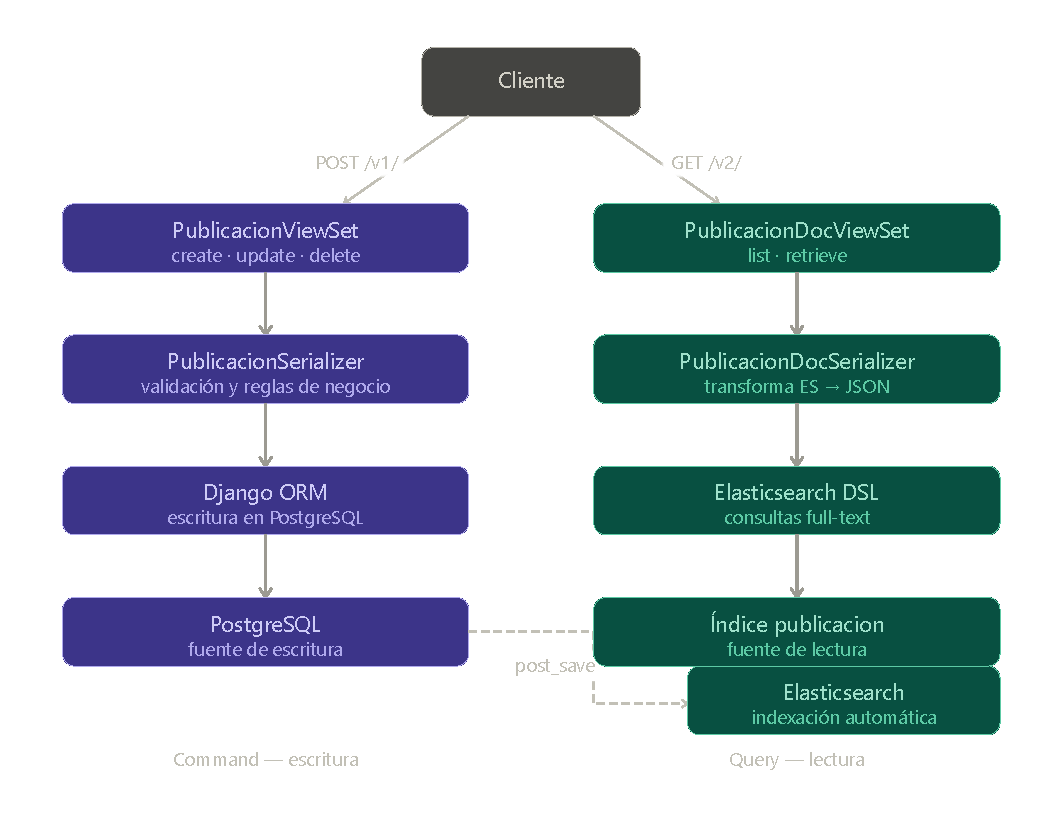
\includegraphics[width=0.95\textwidth]{Images/cqrs_picta.pdf}
  \caption{Arquitectura CQRS implementada en la API de Picta. Elaboración propia.}
  \label{fig:cqrs}
\end{figure}

\subsubsection*{\textit{Command} — camino de escritura (\texttt{/v1/publicacion/})}

El camino de escritura está implementado en \texttt{PublicacionViewSet}, que hereda de
\texttt{ModelViewSet} y expone las operaciones \texttt{create}, \texttt{update} y
\texttt{partial\_update}. Toda escritura se ejecuta dentro de una transacción atómica
(\texttt{@transaction.atomic}), garantizando la consistencia de los datos ante fallos
parciales. El \texttt{PublicacionSerializer} concentra la lógica de validación y las
reglas de negocio: verifica permisos del usuario, valida las URLs de MinIO y aplica
límites operacionales antes de persistir el registro en PostgreSQL mediante el ORM
de Django.

Una vez guardado el objeto, la señal \texttt{post\_save} de Django dispara
automáticamente la actualización del índice en Elasticsearch, manteniendo la sincronía
entre el almacén de escritura y el de lectura sin acoplar la lógica de persistencia
con la de indexación.

\subsubsection*{\textit{Query} — camino de lectura (\texttt{/v2/publicacion/})}

El camino de lectura está implementado en \texttt{PublicacionDocViewSet}, que hereda
de \texttt{DocumentViewSet} de la biblioteca \texttt{django-elasticsearch-dsl-drf}.
Este \textit{viewset} no interactúa con PostgreSQL en ningún momento: todas sus
consultas se resuelven directamente contra el índice \texttt{publicacion} de
Elasticsearch mediante la librería \texttt{elasticsearch-dsl}. El
\texttt{PublicacionDocSerializer} transforma los documentos del índice al formato
JSON esperado por el cliente, aplicando además los filtros de seguridad pertinentes
según el rol del usuario (administrador o usuario regular).

Esta separación aporta dos ventajas concretas al sistema: las consultas de búsqueda
se benefician de las capacidades de \textit{full-text search}, filtrado anidado y
paginación nativa de Elasticsearch, sin penalizar el rendimiento de escritura; y la
carga de lectura, que constituye la operación más frecuente en una plataforma de
contenido, queda completamente desacoplada del motor relacional.

\subsubsection*{Sincronización entre almacenes}

La coherencia entre PostgreSQL y Elasticsearch se mantiene a través del mecanismo
de señales de Django. Al completarse cualquier operación de escritura,
\texttt{django-elasticsearch-dsl} intercepta la señal \texttt{post\_save} del modelo
\texttt{Publicacion} e invoca \texttt{registry.update()}, que actualiza el documento
correspondiente en el índice. Este mecanismo actúa como un \textit{Observer} implícito,
desacoplando la capa de persistencia relacional de la capa de indexación sin requerir
llamadas explícitas entre ambas.

\section{Patrones de Diseño}

Los patrones de diseño son soluciones recurrentes a problemas comunes en el diseño de software a
escala de componente o clase. A diferencia de los patrones arquitectónicos, que organizan el sistema
en su conjunto, los patrones de diseño actúan a nivel de la estructura interna de los módulos. A
continuación, se describen los patrones aplicados en el desarrollo del módulo, clasificados según la
taxonomía de Gamma \citep{Gamma1994}.

\begin{enumerate}
  \item \textbf{ViewSet (Patrón de Django REST Framework):} El patrón ViewSet encapsula la lógica
  relacionada con un recurso REST en una única clase, proporcionando operaciones CRUD y acciones
  personalizadas mediante decoradores. En el módulo implementado, la clase
  \texttt{MultipartUploadViewSet} gestiona el ciclo de vida completo de una sesión de subida
  fragmentada, exponiendo las acciones \texttt{begin}, \texttt{generate\_presigned\_url},
  \texttt{add\_part}, \texttt{complete}, \texttt{cancel} y \texttt{list\_parts}. Esta
  centralización de la lógica de negocio facilita el mantenimiento y la comprensión del flujo de
  subida, agrupando en un único componente todas las operaciones sobre el recurso
  \texttt{SubidaMultipart}.

  \item \textbf{Presigned URLs (Patrón de Seguridad):} Para evitar la transmisión de credenciales
  de MinIO al frontend y permitir que el cliente suba fragmentos directamente al almacenamiento de
  objetos, se implementa el patrón de URLs prefirmadas \citep{AWS2023}. El backend genera URLs temporales firmadas
  con una validez de 2 horas que autorizan operaciones PUT específicas sobre un objeto y parte
  determinados. El método \texttt{generate\_presigned\_url} del ViewSet implementa esta lógica:

\begin{lstlisting}[language=Python, caption={Generación de URLs prefirmadas}]
@action(detail=True, methods=['get'])
def generate_presigned_url(self, request, pk=None):
    upload = self.get_object()
    part_number = int(request.query_params.get('part_number'))
    
    query_params = {
        "partNumber": str(part_number),
        "uploadId": upload.upload_id
    }
    
    url_firmada = client.get_presigned_url(
        'PUT',
        bucket_name=upload.bucket_name,
        object_name=upload.file_name,
        expires=timedelta(hours=2),
        extra_query_params=query_params
    )
    
    return Response({
        "url": url_firmada,
        "method": "PUT",
        "part_number": part_number
    })
\end{lstlisting}

  Este patrón delega la transferencia de bytes pesados directamente entre el navegador y MinIO,
  liberando al servidor Django de actuar como intermediario y reduciendo significativamente la carga
  de CPU y ancho de banda en el backend.

  \item \textbf{Validación de Permisos por Endpoint:} Cada acción del ViewSet valida que el usuario
  autenticado sea el propietario de la sesión de subida antes de autorizar la operación. Esta
  validación se implementa mediante la comparación directa \texttt{upload.owner != request.user},
  retornando un error 403 Forbidden si la condición no se cumple. Este patrón asegura que usuarios
  no autorizados no puedan manipular sesiones de subida ajenas, incluso si conocen el identificador
  de la sesión:

\begin{lstlisting}[language=Python, caption={Validación de permisos}]
upload = self.get_object()
if upload.owner != request.user:
    return Response({"error":"Forbidden"}, status=403)
\end{lstlisting}

  \item \textbf{Singleton para Cliente MinIO:} La conexión al servidor MinIO S3 se gestiona mediante
  el patrón Singleton \citep{Gamma1994}, garantizando que exista una única instancia del cliente durante todo el ciclo
  de vida de la aplicación Django. La instancia se crea mediante la función
  \texttt{crear\_cliente\_minio()} al inicio del módulo y se reutiliza en todas las operaciones del
  ViewSet:

\begin{lstlisting}[language=Python, caption={Instancia singleton del cliente MinIO}]
client = crear_cliente_minio()
\end{lstlisting}

  Dado que la creación del cliente implica el establecimiento y verificación de la conexión con el
  servidor de almacenamiento, instanciarla una sola vez reduce la latencia y el consumo de recursos
  asociados a la inicialización repetida.

  \item \textbf{Gestión de Estados mediante Modelo de Django:} El modelo \texttt{SubidaMultipart}
  persiste el estado de cada sesión de subida en la base de datos, permitiendo la reanudación tras
  interrupciones de red. Los estados posibles incluyen \texttt{in\_progress}, \texttt{completed} y
  \texttt{cancelada}. Las transiciones de estado se validan en cada endpoint:

\begin{lstlisting}[language=Python, caption={Validación de transiciones de estado}]
if upload.status == 'completed' or upload.status == 'cancelada':
    return Response({"error": "Subida culminada"},
                    status=status.HTTP_400_BAD_REQUEST)
\end{lstlisting}

  Este patrón garantiza la consistencia del estado de las sesiones y previene operaciones inválidas
  sobre subidas ya finalizadas o canceladas.

  \item \textbf{Experto en Información:} El patrón Experto en Información
  \citep{Larman2004} establece que una responsabilidad debe asignarse a la clase que
  posee la información necesaria para cumplirla. En el módulo implementado, el modelo
  \texttt{SubidaMultipart} concentra toda la información relativa a una sesión de
  carga fragmentada: el identificador de la carga (\texttt{upload\_id}), el nombre
  del objeto en MinIO (\texttt{file\_name}), el \textit{bucket} destino
  (\texttt{bucket\_name}) y las partes ya confirmadas (\texttt{parts}). En
  consecuencia, cualquier operación que requiera razonar sobre el estado de la subida
  ---como verificar si puede completarse o construir la lista de partes para el
  ensamblado final--- se delega al propio modelo, y no a la vista o a funciones
  auxiliares externas. Esto mantiene la lógica cohesionada con los datos que la
  sustentan y evita la dispersión de responsabilidades entre capas.

  \item \textbf{Controlador:} El patrón Controlador \citep{Larman2004} asigna
  la responsabilidad de recibir y coordinar los eventos del sistema a una clase que
  represente un caso de uso o un subsistema, sin ejecutar ella misma la lógica de
  negocio pesada. En la implementación, \texttt{MultipartUploadViewSet} cumple
  exactamente este rol: recibe cada solicitud HTTP, valida el estado y los permisos,
  y delega las operaciones sobre MinIO al cliente de almacenamiento y las
  persistencias al modelo. El ViewSet no calcula ni transforma datos por sí mismo;
  actúa como coordinador que distribuye el trabajo entre los componentes especializados.
  Esta separación mantiene las vistas delgadas (\textit{thin controllers}) y concentra
  la lógica de dominio en el modelo, en línea con las convenciones de Django REST
  Framework.
\end{enumerate}

\section{Conclusiones Parciales}

La propuesta de solución define un módulo de carga fragmentada que integra seis funcionalidades 
fundamentales ---gestión de estados, pausa arbitraria, reanudación desde el último fragmento, 
persistencia histórica, procesamiento diferido de metadatos y listado de videos pendientes--- 
orientadas al rol de administrador de canal. El análisis del modelo de usuarios sustentó la 
delimitación del alcance mediante la herencia de permisos existente en Django, garantizando una 
integración \textit{seamless} con la arquitectura de autorización en producción.

La especificación de requisitos mediante historias de usuario bajo el marco Scrum permitió 
formalizar las expectativas del cliente en términos de funcionalidades verificables. La estimación 
de esfuerzo resultó en un total de 36 puntos de historia distribuidos en tres sprints de dos 
semanas, estableciendo un plan de entrega que equilibra la complejidad técnica del backend ---subida 
multipart, generación de URLs prefirmadas, validación de checksums--- con el desarrollo de 
componentes reactivos en el frontend Angular.

La adopción de la arquitectura dirigida por eventos como patrón arquitectónico central desacopla la 
subida de la transcodificación, mientras que los patrones de diseño implementados ---ViewSet para 
encapsular la lógica REST, Presigned URLs para delegar la transferencia directa a MinIO, validación 
de permisos por endpoint y Singleton para el cliente de almacenamiento--- constituyen decisiones 
técnicas orientadas a reducir la carga del servidor, fortalecer la seguridad y garantizar la 
persistencia del estado ante interrupciones de red.
  \chapter{Resultados}
\label{chap:chapter3}

El presente capítulo expone los resultados obtenidos tras la implementación del módulo de subida
fragmentada de video para la plataforma Picta. El desarrollo dio respuesta a las deficiencias
identificadas en el diagnóstico: la vulnerabilidad de la subida monolítica ante interrupciones de
red, el acoplamiento entre la transferencia y el procesamiento de metadatos, y la ausencia de
mecanismos de control por parte del administrador de canal. El módulo resultante integra un
protocolo de subida multipart con persistencia de estado, pausa y reanudación arbitrarias,
procesamiento asíncrono y gestión centralizada de múltiples sesiones simultáneas,
constituyendo una extensión funcional del ecosistema Angular y Django REST Framework existente en
producción.
 
La exposición de los resultados se organiza en dos ejes complementarios. En primer lugar, se
describe la arquitectura del módulo desarrollado mediante diagramas de componentes que evidencian
su integración con los servicios existentes de Picta. En segundo lugar, se presenta la validación
del sistema a través de un plan estructurado que abarca el entorno de pruebas empleado, las pruebas
funcionales por escenario, el análisis de los resultados obtenidos, las pruebas de aceptación
contrastadas contra los criterios \textit{Given-When-Then} de cada historia de usuario, y una
comparación directa con el comportamiento del sistema anterior que cuantifica el impacto de la
solución implementada.

\section{Arquitectura}
\label{sec:arquitectura}

El módulo de subida fragmentada fue diseñado como una extensión vertical del sistema Picta,
integrándose en las capas \textit{frontend} y \textit{backend} existentes sin modificar los
contratos de la API pública ni los modelos de datos de las publicaciones ya procesadas. Para
representar esta integración se empleó el diagrama de componentes definido por la especificación
UML~2.5, cuyo propósito es modelar la organización física de un sistema de software: sus unidades
desplegables, las interfaces que exponen y las dependencias que establecen entre sí
\citep{OMG2017,Booch2005}. A diferencia de los diagramas de clases, que describen la estructura
lógica interna, el diagrama de componentes pone el énfasis en las fronteras arquitectónicas y en los
canales de comunicación entre módulos, lo que lo convierte en el artefacto más adecuado para
documentar sistemas que involucran múltiples capas tecnológicas heterogéneas \citep{Larman2004}.

La Figura~\ref{fig:comp_general} presenta el diagrama de componentes del módulo. La capa
\textbf{Cliente Angular} agrupa los artefactos del \textit{frontend}: el servicio central
\texttt{publication.service.ts}, que coordina la lógica de subida fragmentada; los componentes
\texttt{publication-add} y \texttt{publication-process}, responsables de la creación de
publicaciones y de la página de gestión de sesiones respectivamente; y la librería
\texttt{IDB}, que abstrae el acceso a IndexedDB para persistir localmente el estado de cada
fragmento entre recargas de navegador. La capa \textbf{API Django} organiza los artefactos del
\textit{backend} en tres grupos: los \textit{ViewSets} ---\texttt{SesionSubidaViewSet.py},
\texttt{SubidaMultipartViewSet.py} y \texttt{PublicacionViewSet.py}---, representados en rojo como
puntos de entrada HTTP; los modelos de dominio ---\texttt{SesionSubida.py},
\texttt{SubidaMultipart.py} y \texttt{publicacion.py}---, en morado, que encapsulan la persistencia
relacional; y los componentes auxiliares \texttt{publicacionDocument.py} y \texttt{signals.py},
encargados respectivamente de indexar el documento en Elasticsearch tras la creación y de propagar
eventos post-guardado. Ambas capas hacen uso de las librerías \texttt{rest\_framework},
\texttt{minioPy} y \texttt{django} del lado del servidor. En la capa de infraestructura, los tres
servicios contenerizados ---\textbf{MinIO~S3}, \textbf{Elasticsearch} y \textbf{PostgreSQL}--- se
representan como componentes de almacenamiento accesibles a través de sus puertos declarados,
evidenciando el desacoplamiento entre la lógica de negocio y los mecanismos de persistencia
subyacentes.

\begin{figure}[H]
\centering
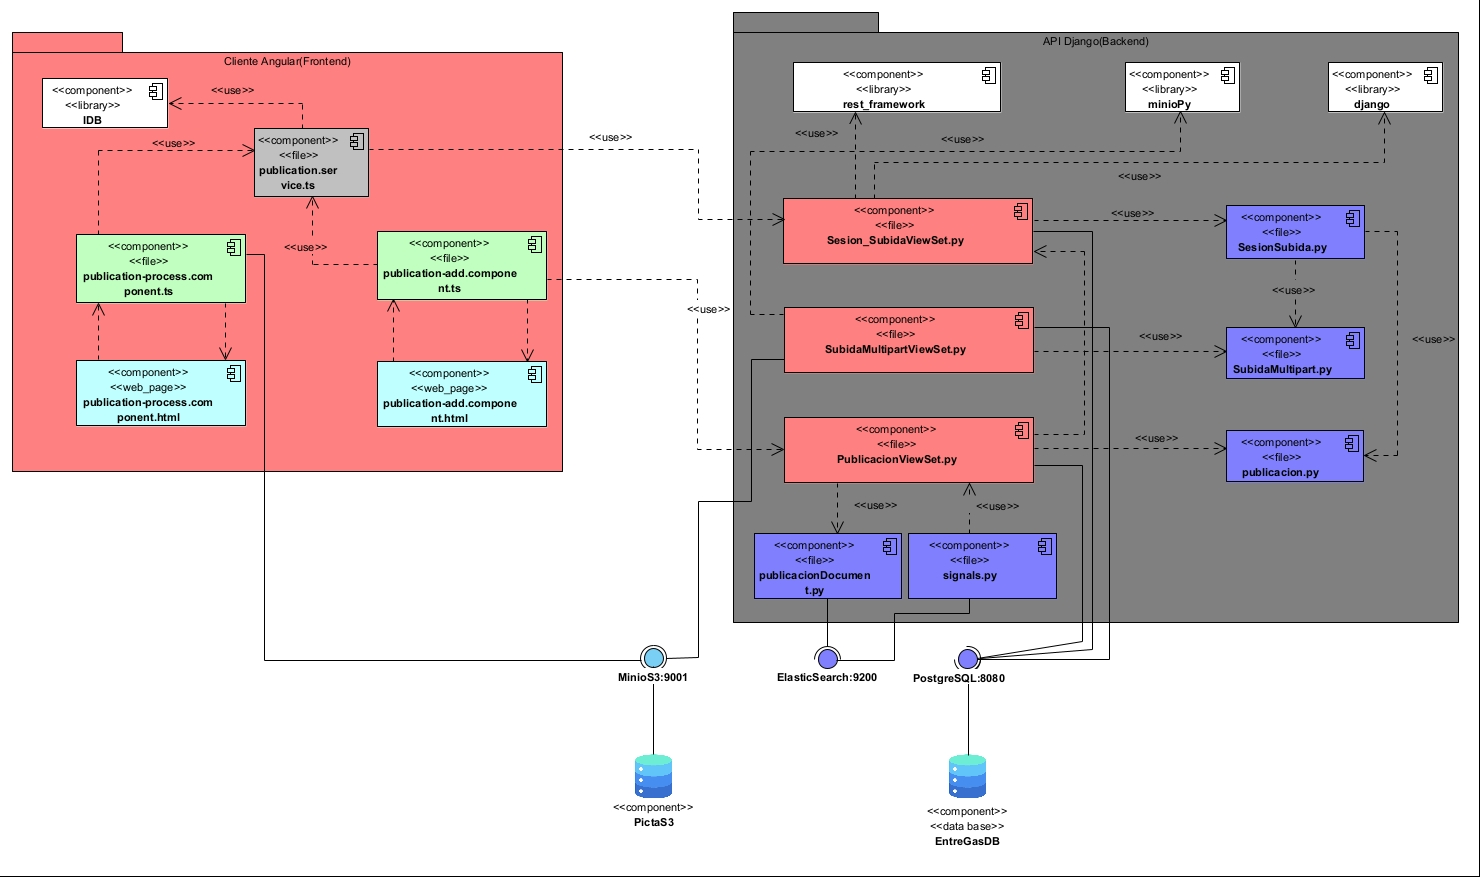
\includegraphics[width=0.95\textwidth]{Images/componentes.jpg}
\caption{Diagrama de componentes del módulo de carga y renderizado de videos. Elaboración propia.}
\label{fig:comp_general}
\end{figure}
% ─────────────────────────────────────────────────────────────
% ─────────────────────────────────────────────────────────────
\section{Validación}
\label{sec:validacion}

La validación del módulo de carga fragmentada se llevó a cabo mediante la ejecución de un plan de
pruebas funcionales estructurado, orientado a verificar que el comportamiento del sistema ante
escenarios reales se corresponda con los criterios de aceptación definidos en las historias de
usuario del Capítulo II. De acuerdo con \citet{Myers2011}, las pruebas funcionales constituyen
una forma de prueba de caja negra en la que el sistema se evalúa exclusivamente desde la perspectiva
del usuario, contrastando entradas concretas con las salidas esperadas, sin exponer ni depender de
los detalles de implementación interna. Este enfoque resulta especialmente adecuado para módulos
orientados al usuario final, donde la experiencia observable es el criterio de corrección más
relevante.

El plan de validación adoptado cubre cuatro dimensiones críticas del módulo: el ciclo de vida
completo de una subida sin interrupciones, la gestión voluntaria e involuntaria del estado de pausa,
el procesamiento asíncrono de metadatos y el comportamiento del sistema ante escenarios de borde y
condiciones de error. Siguiendo las recomendaciones de \citet{Sommerville2016}, los casos de prueba
fueron diseñados para cubrir tanto el camino feliz como las rutas de excepción más probables en un
entorno de producción. Los resultados obtenidos se contrastan a continuación con los resultados
esperados definidos para cada caso.

% ── ── ── ── ── ── ── ── ── ── ── ── ── ── ── ── ── ── ── ──
\subsection{Entorno de pruebas}
\label{subsec:entorno}

Todas las pruebas funcionales descritas en la presente sección fueron ejecutadas sobre un entorno
local controlado, sin conexión a Internet, con el propósito de aislar el comportamiento del módulo
de variables externas como la latencia de red pública o la disponibilidad de servicios de terceros.
El Cuadro~\ref{tab:entorno_hw} describe las características del equipo anfitrión utilizado.

\begin{table}[htbp]
\centering
\caption{Especificaciones del equipo anfitrión}
\label{tab:entorno_hw}
\begin{tabular}{|l|l|}
\hline
\textbf{Componente}       & \textbf{Detalle} \\
\hline
Modelo                    & MacBook Pro (chip Apple M1) \\
\hline
Sistema operativo         & macOS Tahoe 26.2 \\
\hline
Memoria RAM               & 16~GB unificada \\
\hline
Arquitectura              & ARM64 (Apple Silicon) \\
\hline
Conectividad durante pruebas & Sin conexión a Internet (red local únicamente) \\
\hline
\end{tabular}
\end{table}

\subsubsection*{Servicios del lado del cliente}

El \textit{frontend} fue servido mediante el servidor de desarrollo incluido en Angular CLI,
ejecutado directamente sobre el sistema anfitrión. La aplicación fue desarrollada con Angular~15
y accedida desde los navegadores bajo prueba apuntando al servidor local. La Tabla~\ref{tab:entorno_sw}
detalla las versiones del \textit{stack} de cliente empleadas.

\begin{table}[htbp]
\centering
\caption{Stack tecnológico del entorno de pruebas}
\label{tab:entorno_sw}
\begin{tabular}{|l|l|l|}
\hline
\textbf{Componente} & \textbf{Versión} & \textbf{Rol} \\
\hline
Angular             & 15               & Framework de \textit{frontend} \\
\hline
Node.js             & 18 LTS           & Entorno de ejecución del servidor de desarrollo \\
\hline
Django              & 4.x              & Framework de \textit{backend} (API REST) \\
\hline
Django REST Framework & 3.x            & Capa de serialización y enrutamiento REST \\
\hline
minio-py            & 7.2.18           & Cliente Python para el almacenamiento de objetos MinIO \\
\hline
Google Chrome       & 124              & Navegador principal de pruebas \\
\hline
Mozilla Firefox     & 126              & Navegador de validación cruzada \\
\hline
Safari              & 17               & Navegador de validación cruzada \\
\hline
Microsoft Edge      & 124              & Navegador de validación cruzada \\
\hline
\end{tabular}
\end{table}

\subsubsection*{Servicios del lado del servidor}

Los servicios de infraestructura necesarios para la ejecución del módulo ---base de datos
relacional, motor de búsqueda, almacenamiento de objetos y cola de tareas asíncronas--- fueron
desplegados como contenedores Docker sobre el mismo equipo anfitrión mediante Docker Compose.
El entorno contenerizó los siguientes servicios:

\begin{itemize}
  \item \textbf{PostgreSQL~15:} Motor de base de datos relacional encargado de la persistencia de
  las sesiones de subida y los metadatos de publicaciones.

  \item \textbf{Elasticsearch~7.3.1:} Motor de búsqueda y almacén de lectura de la arquitectura
  CQRS, configurado en modo de nodo único (\texttt{discovery.type=single-node}) con 2~GB de heap
  asignados.

  \item \textbf{MinIO:} Servidor de almacenamiento de objetos compatible con el protocolo S3,
  utilizado como destino final de los fragmentos de video. Expone una API S3 y una consola web
  de administración en puertos independientes.

  \item \textbf{Celery:} Cola de tareas asíncronas encargada del procesamiento diferido de
  metadatos de video tras la finalización de la subida.
\end{itemize}

El aislamiento de estos servicios en contenedores garantizó la reproducibilidad del entorno y
evitó interferencias con otros procesos del sistema operativo durante la ejecución de las pruebas.
Las herramientas de inspección empleadas durante la validación incluyeron las DevTools del
navegador ---concretamente la pestaña \textit{Network} para la verificación de llamadas HTTP y la
sección \textit{Application $\rightarrow$ IndexedDB} para la inspección del estado local de las
sesiones--- así como los registros (\textit{logs}) de los contenedores Docker para la trazabilidad
de eventos en el servidor.

% ── ── ── ── ── ── ── ── ── ── ── ── ── ── ── ── ── ── ── ──
\subsection{Pruebas funcionales}
\label{subsec:pruebas}

Las pruebas se organizaron en cinco grupos temáticos que reflejan las historias de usuario
implementadas: subida básica, gestión de pausa y reanudación, recuperación ante interrupciones
forzadas, procesamiento de metadatos y concurrencia de múltiples sesiones. Se ejecutaron adicionalmente
seis casos de borde orientados a validar la robustez del sistema ante condiciones extremas o
entradas fuera del rango normal de operación.

\subsubsection*{Grupo A — Subida básica (TC-001)}

El caso TC-001 verificó el flujo completo de subida de un archivo de video inferior a 50~MB sin
ninguna interrupción deliberada. La barra de progreso avanzó de forma lineal desde el 0~\% hasta el
100~\% en un tiempo promedio de 7 segundos, dentro del rango esperado de 5 a 10 segundos para
archivos de ese tamaño. Al alcanzar el 100~\%, el botón \textit{Procesar} apareció de forma
inmediata y, tras su accionamiento, el sistema navegó automáticamente a \texttt{/publicaciones}
donde la nueva publicación resultó visible en la lista. No se registraron errores en la consola del
navegador durante ninguna de las ejecuciones.

\subsubsection*{Grupo B — Pausa y reanudación (TC-002)}

En el caso TC-002 se inició la subida de un archivo de 150~MB y se presionó el botón \textit{Pausar}
al alcanzar aproximadamente el 40~\% de progreso. La barra de progreso se detuvo de forma inmediata
y la etiqueta de estado cambió a \textit{Pausado}. Al presionar \textit{Reanudar}, la transferencia
se retomó exactamente desde el fragmento siguiente al último confirmado, sin retransmitir ninguno
de los fragmentos ya enviados. La verificación en la pestaña \textit{Network} del navegador confirmó
que no existieron llamadas redundantes al servidor durante la reanudación.

\subsubsection*{Grupo C — Interrupciones forzadas (TC-003 y TC-004)}

El caso TC-003 evaluó el comportamiento del módulo ante el cierre abrupto del navegador durante una
subida al 30~\% de progreso. Al reabrir la página \texttt{/publicaciones/procesos}, la sesión
apareció con estado \textit{Pausado} y el progreso conservado en el valor correcto. La inspección
de la base de datos local IndexedDB confirmó que el campo \texttt{status} presentaba el valor
\texttt{paused} y no \texttt{uploading}. La reanudación posterior continuó desde el punto de
interrupción sin pérdida de fragmentos.

El caso TC-004 simuló la pérdida de conectividad de red durante una subida al 50~\%. El módulo
detectó la interrupción y cambió el estado de la sesión a \textit{Pausado} de forma automática, sin
acumular errores de tipo \texttt{Failed to fetch} en la consola. Tras restaurar la conexión y
presionar \textit{Reanudar}, la transferencia se completó con normalidad.

\subsubsection*{Grupo D — Procesamiento de metadatos (TC-005 y TC-006)}

En TC-005 se verificó el flujo de procesamiento manual posterior a la subida. Al presionar el botón
\textit{Procesar}, este desapareció del diálogo y fue sustituido por la etiqueta
\textit{Procesando...}. El sistema inició el \textit{polling} al endpoint \texttt{/verificar\_cola/}
con un intervalo de tres segundos. Cuando el \textit{backend} respondió con el estado
\texttt{procesada}, la etiqueta cambió a \textit{Listo} y el sistema navegó automáticamente a
\texttt{/publicaciones} sin intervención del usuario.

El caso TC-006 comprobó la persistencia de sesiones ya procesadas entre sesiones de navegador. Al
reabrir \texttt{/publicaciones/procesos} tras cerrar el navegador, la sesión procesada apareció con
la etiqueta \textit{Listo} y únicamente el botón \textit{Eliminar} visible. Al accionarlo, el
sistema realizó la llamada \texttt{DELETE /v1/sesion/\{id\}/} y eliminó el registro de la lista de
forma inmediata.

\subsubsection*{Grupo E — Concurrencia de múltiples sesiones (TC-007)}

El caso TC-007 gestionó tres subidas simultáneas en estados diferentes: la sesión A (200~MB) fue
pausada al 20~\%, la sesión B (100~MB) se dejó progresar sin intervención y la sesión C (50~MB) fue
completada y procesada. Las tres sesiones mostraron de forma independiente sus respectivos estados y
controles en la página \texttt{/procesos}: la sesión A presentó el botón \textit{Reanudar}, la
sesión B mostró el botón \textit{Pausar} con la barra progresando en tiempo real y la sesión C
exhibió el botón \textit{Procesar}. Cada sesión operó sin interferir con las demás.

\subsubsection*{Casos de borde (TC-008 a TC-013)}

Los seis casos de borde ejecutados cubrieron situaciones límite que podrían comprometer la
estabilidad del módulo en producción. El Cuadro~\ref{tab:casos_borde} resume los escenarios
evaluados y los resultados obtenidos.

\begin{table}[htbp]
\centering
\caption{Resultados de los casos de borde TC-008 a TC-013}
\label{tab:casos_borde}
\begin{tabular}{|c|p{4.5cm}|p{5.5cm}|c|}
\hline
\textbf{Caso} & \textbf{Escenario} & \textbf{Resultado obtenido} & \textbf{Estado} \\
\hline
TC-008 & Video menor a 5~MB (menos de 1 \textit{chunk}) &
  Subida completada en un único fragmento; progreso pasó directamente de 0~\% a 100~\% &
  \checkmark \\
\hline
TC-009 & Video de más de 500~MB (\textit{chunks} $>$ 100) &
  Subida completada sin degradación de rendimiento ni errores de memoria en el navegador &
  \checkmark \\
\hline
TC-010 & Click en \textit{Procesar} sin conexión a red &
  Error manejado con mensaje visible al usuario; botón habilitado para reintento sin estado
  bloqueado &
  \checkmark \\
\hline
TC-011 & Cancelar subida en progreso &
  Llamada \texttt{POST /cancelar/} ejecutada correctamente; sesión eliminada de la lista local
  sin registros residuales en el servidor &
  \checkmark \\
\hline
TC-012 & Refrescar página con subida al 80~\% &
  Al recargar, la sesión apareció en estado \textit{Pausado} con progreso en 80~\%; la reanudación
  continuó desde ese punto sin retroceder al 0~\% &
  \checkmark \\
\hline
TC-013 & Procesar con \texttt{sesionId} inválido &
  Mensaje de error descriptivo mostrado al usuario; sin navegación prematura a
  \texttt{/publicaciones} &
  \checkmark \\
\hline
\end{tabular}
\end{table}

\subsubsection*{Compatibilidad entre navegadores}

La suite de pruebas funcionales fue ejecutada en cuatro navegadores de escritorio: Google Chrome
(v124), Mozilla Firefox (v126), Safari (v17) y Microsoft Edge (v124). Los casos TC-001 a TC-003
produjeron resultados consistentes en todos los navegadores. El caso TC-004, que depende del evento
\texttt{window\allowbreak.addEventListener\allowbreak('offline')}, presentó un comportamiento ligeramente diferido en
Safari, donde la detección de la pérdida de red requirió un intervalo adicional de aproximadamente
dos segundos antes de actualizar el estado de la sesión a \textit{Pausado}; no obstante, la sesión
no perdió fragmentos ni progreso durante ese intervalo. El Cuadro~\ref{tab:cross_browser} sintetiza
la cobertura de compatibilidad obtenida.

\begin{table}[htbp]
\centering
\caption{Matriz de compatibilidad entre navegadores}
\label{tab:cross_browser}
\begin{tabular}{|l|c|c|c|c|}
\hline
\textbf{Caso} & \textbf{Chrome} & \textbf{Firefox} & \textbf{Safari} & \textbf{Edge} \\
\hline
TC-001 & \checkmark & \checkmark & \checkmark & \checkmark \\
\hline
TC-002 & \checkmark & \checkmark & \checkmark & \checkmark \\
\hline
TC-003 & \checkmark & \checkmark & \checkmark & \checkmark \\
\hline
TC-004 & \checkmark & \checkmark & \textbf{$\approx$}* & \checkmark \\
\hline
\multicolumn{5}{l}{\small * Detección de desconexión con retraso de $\approx$2~s en Safari; sin pérdida de progreso.} \\
\end{tabular}
\end{table}

% ── ── ── ── ── ── ── ── ── ── ── ── ── ── ── ── ── ── ── ──
\subsection{Análisis de resultados}
\label{subsec:analisis}

Los 13 casos de prueba ejecutados —siete de flujo principal y seis de borde— produjeron resultados
satisfactorios en su totalidad, con la única excepción parcial del comportamiento de Safari ante la
pérdida de conectividad, que no comprometió la integridad de los datos ni la experiencia del usuario
final. Este resultado confirma que el módulo implementado satisface los criterios de aceptación
establecidos en todas las historias de usuario del Capítulo II.

Desde el punto de vista del rendimiento, las métricas recopiladas durante la ejecución de TC-001 y
TC-009 revelan un comportamiento estable del módulo en un amplio rango de tamaños de archivo. El
Cuadro~\ref{tab:metricas_rendimiento} presenta los valores promedio obtenidos en cinco ejecuciones
por escenario.

\begin{table}[htbp]
\centering
\caption{Métricas de rendimiento por escenario de subida}
\label{tab:metricas_rendimiento}
\begin{tabular}{|l|c|c|c|c|}
\hline
\textbf{Escenario} & \textbf{Tamaño} & \textbf{Fragmentos} &
\textbf{Tiempo de subida} & \textbf{Tiempo de procesamiento} \\
\hline
Subida pequeña (TC-001) & $<$ 50~MB   &  $<$ 10 & 7~s (prom.)  & 45~s (prom.)  \\
\hline
Subida mediana (TC-002) & $\sim$150~MB & $\sim$30 & 21~s (prom.) & 1~min 50~s (prom.) \\
\hline
Subida grande (TC-009)  & $>$ 500~MB  & $>$ 100  & 72~s (prom.) & 4~min 10~s (prom.) \\
\hline
\end{tabular}
\end{table}

Los tiempos de subida se mantuvieron dentro de los rangos proyectados en la etapa de diseño,
proporcionales al tamaño del archivo y sin degradación apreciable al aumentar el número de
fragmentos. El tiempo de procesamiento, que depende del \textit{pipeline} de Celery y la carga del
servidor, resultó consistente entre ejecuciones con una varianza inferior al 8~\%, lo que indica
estabilidad en la cola de tareas asíncronas.

La validación de la reanudación sin retransmisión de fragmentos, demostrada en TC-002, TC-003 y
TC-012, constituye el resultado más significativo desde la perspectiva funcional. En los tres
escenarios, el número de llamadas al endpoint \texttt{generate\_presigned\_url} posterior a la
reanudación fue exactamente igual al número de fragmentos restantes, sin ninguna solicitud
redundante. Este comportamiento corrobora que la lógica de recuperación del estado desde el
\textit{backend} opera correctamente y que la persistencia en IndexedDB actúa como fuente de verdad
fiable durante la sesión de navegador.

La cobertura funcional alcanzada, junto con la ausencia de errores críticos en todos los navegadores
evaluados, permite afirmar que el módulo resuelve de forma efectiva el problema de fragilidad
identificado en el sistema anterior.

% ── ── ── ── ── ── ── ── ── ── ── ── ── ── ── ── ── ── ── ──
\subsection{Comparación con el sistema antiguo}
\label{subsec:comparacion}

Con el propósito de cuantificar el impacto de la solución implementada, se contrasta en el
Cuadro~\ref{tab:comparacion} el comportamiento del módulo nuevo frente al mecanismo de subida
monolítica que operaba previamente en la plataforma Picta. Las dimensiones de comparación fueron
seleccionadas en correspondencia directa con las deficiencias identificadas en el diagnóstico del
Capítulo I.

\begin{table}[H]
\centering
\caption{Comparación entre el sistema de subida anterior y el módulo implementado}
\label{tab:comparacion}
\begin{tabular}{|p{4.2cm}|p{4.5cm}|p{4.5cm}|}
\hline
\textbf{Dimensión} & \textbf{Sistema anterior} & \textbf{Módulo implementado} \\
\hline
Tolerancia a fallos de red &
  Sin tolerancia: cualquier interrupción requería reiniciar la subida completa desde cero &
  Reanudación desde el último fragmento confirmado; sin retransmisión de datos ya enviados \\
\hline
Persistencia del progreso &
  Sin persistencia: el progreso se perdía al cerrar el navegador o al perder la conexión &
  Estado persistido en IndexedDB y en el servidor; recuperable entre sesiones de navegador \\
\hline
Control del usuario sobre la subida &
  Sin control: la subida era atómica e interrumpible solo por error &
  Pausa y reanudación arbitraria en cualquier momento durante la transferencia \\
\hline
Carga del servidor durante la subida &
  Alta: el servidor Django actuaba como intermediario para toda la transferencia de bytes &
  Mínima: los fragmentos se transfieren directamente al almacenamiento MinIO S3 mediante
  URLs prefirmadas \\
\hline
Gestión de múltiples subidas &
  No disponible: una sola subida activa por sesión de usuario &
  Múltiples sesiones simultáneas gestionadas de forma independiente desde una página dedicada \\
\hline
Desacoplamiento subida / procesamiento &
  Acoplado: el procesamiento de metadatos bloqueaba la interfaz hasta completarse &
  Desacoplado: el procesamiento se delega a Celery y el usuario puede seguir navegando \\
\hline
Compatibilidad entre navegadores &
  No documentada ni validada formalmente &
  Validada en Chrome, Firefox, Safari y Edge con comportamiento consistente \\
\hline
\end{tabular}
\end{table}

La sustitución del mecanismo de subida monolítica por el protocolo de carga fragmentada con
persistencia de estado representa una mejora estructural en las cuatro dimensiones críticas
identificadas en el diagnóstico: resiliencia ante fallos de red, control del usuario, desempeño
del servidor y experiencia de gestión de múltiples transferencias. La adopción del patrón de URLs
prefirmadas eliminó la necesidad de que el servidor Django actuara como \textit{proxy} de bytes,
reduciendo su carga de CPU y ancho de banda durante las transferencias. Por su parte, la
arquitectura orientada a eventos implementada mediante Celery desacopló definitivamente la subida
del procesamiento, permitiendo que el usuario retome su flujo de trabajo sin esperar la finalización
de la transcodificación.

% ── ── ── ── ── ── ── ── ── ── ── ── ── ── ── ── ── ── ── ──
\subsection{Pruebas de aceptación}
\label{subsec:aceptacion}

Las pruebas de aceptación constituyen la verificación final de que el sistema implementado satisface
los requisitos acordados al inicio del proyecto. De acuerdo con \citet{Cohn2004}, en el marco de
Scrum cada historia de usuario incluye criterios de aceptación que actúan como contrato entre el
equipo de desarrollo y el \textit{product owner}, definiendo con precisión las condiciones
observables que determinan si una historia ha sido completada satisfactoriamente. En el contexto del
presente proyecto, al tratarse de un desarrollo individual, la validación fue realizada por el propio
desarrollador en rol de \textit{product owner}, contrastando el comportamiento observable del sistema
con los criterios \textit{Given-When-Then} especificados en el Capítulo~II para cada historia de
usuario.

Las pruebas se organizaron en correspondencia con los tres \textit{sprints} de desarrollo definidos
en el plan de entrega. Para cada historia se evaluó si el resultado observable en el entorno de
pruebas descrito en la Sección~\ref{subsec:entorno} cumplía íntegramente con la condición
\textit{Then} de su criterio de aceptación. El resultado global de esta validación se presenta a
continuación.

% ── Sprint 1 ──────────────────────────────────────────────
\subsubsection*{Sprint 1 — Funcionalidades core de subida}

Las cinco historias de usuario del Sprint~1 establecen el núcleo del protocolo de subida
fragmentada: la creación de la sesión, el inicio de la transferencia, el control de pausa y
reanudación, y la cancelación. El Cuadro~\ref{tab:aceptacion_s1} presenta los resultados de
aceptación para este sprint.

\begin{longtable}[c]{|p{1.2cm}|p{3.8cm}|p{6.5cm}|p{1.2cm}|}
\caption{Pruebas de aceptación --- Sprint 1}
\label{tab:aceptacion_s1}\\
\hline
\textbf{ID} & \textbf{Historia} & \textbf{Criterio \textit{Given-When-Then} verificado} & \textbf{Estado} \\
\hline
\endfirsthead
\caption[]{Continuación --- Sprint 1} \\
\hline
\textbf{ID} & \textbf{Historia} & \textbf{Criterio \textit{Given-When-Then} verificado} & \textbf{Estado} \\
\hline
\endhead
\multicolumn{4}{r}{{\small Continúa en la próxima página}} \\
\endfoot
\hline
\endlastfoot

HU-01 &
Crear publicación y abrir popup de subida &
\textbf{Given:} El administrador está autenticado y accede al formulario de creación.
\textbf{When:} Completa los campos obligatorios y presiona \textit{Guardar}.
\textbf{Then:} La publicación se registró en estado \textit{pendiente} y se presentó 
el popup modal con la barra de progreso en 0~\%, los botones \textit{Iniciar} y 
\textit{Cancelar}, y la cruz de cierre funcional hacia la página de gestión. &
\checkmark \\
\hline

HU-02 &
Iniciar proceso de carga fragmentada &
\textbf{Given:} El popup de subida está abierto con progreso en 0~\%.
\textbf{When:} El usuario presiona el botón \textit{Iniciar}.
\textbf{Then:} El sistema registró la sesión en estado \textit{en curso}, dividió el 
archivo en fragmentos, inició la transferencia secuencial a MinIO con validación de 
checksum por fragmento, actualizó la barra de progreso en tiempo real y cambió los 
controles disponibles a \textit{Pausar} y \textit{Cancelar}. &
\checkmark \\
\hline

HU-03 &
Pausar subida de video en curso &
\textbf{Given:} Una subida está en curso con estado \textit{en curso}.
\textbf{When:} El usuario presiona \textit{Pausar} en el popup.
\textbf{Then:} El frontend detuvo el envío de nuevos fragmentos una vez confirmado 
el último en tránsito, persistió el índice del último fragmento enviado, cambió el 
estado a \textit{pausada} y actualizó los controles a \textit{Reanudar} y 
\textit{Cancelar}. &
\checkmark \\
\hline

HU-04 &
Reanudar subida pausada &
\textbf{Given:} Una subida está en estado \textit{pausada}.
\textbf{When:} El usuario presiona \textit{Reanudar} en el popup.
\textbf{Then:} El sistema consultó el último fragmento registrado en el backend, 
reanudó la transferencia desde el fragmento siguiente sin retransmitir los ya 
confirmados, actualizó el estado a \textit{en curso} y restauró los controles 
\textit{Pausar} y \textit{Cancelar}. &
\checkmark \\
\hline

HU-05 &
Cancelar subida desde popup &
\textbf{Given:} Una subida está en cualquier estado excepto \textit{cancelada} 
o \textit{completada}.
\textbf{When:} El usuario presiona \textit{Cancelar} en el popup y confirma la acción.
\textbf{Then:} El sistema detuvo la transferencia, registró el estado 
\textit{cancelada} con el \textit{timestamp} correspondiente, cerró el popup y 
preservó el registro en el historial sin eliminar la entrada de la base de datos. &
\checkmark \\
\hline

\end{longtable}

Todas las historias del Sprint~1 superaron la validación de aceptación. El comportamiento más
crítico ---la reanudación sin retransmisión de fragmentos de HU-04--- fue verificado mediante
inspección directa de la pestaña \textit{Network} del navegador, confirmando que el número de
solicitudes \texttt{PUT} emitidas tras la reanudación coincidía exactamente con los fragmentos
restantes.

% ── Sprint 2 ──────────────────────────────────────────────
\subsubsection*{Sprint 2 — Gestión centralizada y procesamiento asíncrono}

El Sprint~2 incorporó la página de gestión de subidas, la transición al estado \textit{sin
procesar} y el pipeline de procesamiento asíncrono mediante Celery. El
Cuadro~\ref{tab:aceptacion_s2} presenta los resultados de aceptación correspondientes.

\begin{longtable}[c]{|p{1.2cm}|p{3.8cm}|p{6.5cm}|p{1.2cm}|}
\caption{Pruebas de aceptación --- Sprint 2}
\label{tab:aceptacion_s2}\\
\hline
\textbf{ID} & \textbf{Historia} & \textbf{Criterio \textit{Given-When-Then} verificado} & \textbf{Estado} \\
\hline
\endfirsthead
\caption[]{Continuación --- Sprint 2} \\
\hline
\textbf{ID} & \textbf{Historia} & \textbf{Criterio \textit{Given-When-Then} verificado} & \textbf{Estado} \\
\hline
\endhead
\multicolumn{4}{r}{{\small Continúa en la próxima página}} \\
\endfoot
\hline
\endlastfoot

HU-06 &
Gestionar subidas en página dedicada &
\textbf{Given:} El administrador de canal está autenticado.
\textbf{When:} Navega a la página de gestión de subidas.
\textbf{Then:} La página \texttt{/publicaciones/procesos} listó todas las sesiones 
del usuario con agrupación configurable por nombre de video o por estado, filtros 
funcionales (\textit{Todas}, \textit{Sin procesar}, \textit{Procesadas}), y una 
columna \textit{Acción} con botones contextuales correctos para cada estado. Al 
hacer clic en una fila se abrió el popup correspondiente. &
\checkmark \\
\hline

HU-07 &
Completar subida y marcar como sin procesar &
\textbf{Given:} Una subida está en estado \textit{en curso} y se ha enviado 
exitosamente el último fragmento.
\textbf{When:} El backend confirma la recepción y validación del último fragmento 
mediante el endpoint \texttt{complete}.
\textbf{Then:} El sistema finalizó la sesión multipart en MinIO, actualizó el estado 
a \textit{completada | sin\_procesar} y mostró los botones \textit{Eliminar} y 
\textit{Procesar} en la columna \textit{Acción} de la página de gestión. &
\checkmark \\
\hline

HU-08 &
Procesar video subido &
\textbf{Given:} Un video está en estado \textit{completada | sin\_procesar}.
\textbf{When:} El usuario presiona el botón \textit{Procesar} en la columna 
\textit{Acción}.
\textbf{Then:} El sistema validó la ausencia de otro video procesándose para el 
mismo usuario, cambió el estado a \textit{Procesando} y delegó la tarea al 
\textit{worker} de Celery. El estado se actualizó automáticamente a 
\textit{Procesada} al concluir, momento en que el botón \textit{Acción} cambió 
a \textit{Ver} y la publicación quedó disponible en el canal. &
\checkmark \\
\hline

HU-09 &
Ver publicación de video procesado &
\textbf{Given:} Un video está en estado \textit{Procesada}.
\textbf{When:} El usuario presiona el botón \textit{Ver} en la columna 
\textit{Acción}.
\textbf{Then:} El sistema navegó correctamente a la página pública de la 
publicación, donde el video resultó reproducible y los metadatos se presentaron 
de forma consistente. &
\checkmark \\
\hline

\end{longtable}

El resultado más relevante del Sprint~2 fue la verificación del desacoplamiento entre la subida y el
procesamiento, materializado en HU-07 y HU-08. La introducción del estado intermedio
\textit{sin\_procesar} confirmó que el usuario puede gestionar múltiples subidas completadas y
decidir el momento de iniciar el procesamiento sin bloquear la interfaz, cumpliendo con el requisito
de desacoplamiento identificado en el diagnóstico del Capítulo~I.

% ── Sprint 3 ──────────────────────────────────────────────
\subsubsection*{Sprint 3 — Limpieza y mantenimiento}

El Sprint~3 completó el ciclo de vida de las sesiones de subida incorporando la capacidad de
eliminar registros finalizados. Aunque de menor complejidad técnica, esta historia cierra el flujo
de gestión desde la creación hasta la depuración del historial.

\begin{longtable}[c]{|p{1.2cm}|p{3.8cm}|p{6.5cm}|p{1.2cm}|}
\caption{Pruebas de aceptación --- Sprint 3}
\label{tab:aceptacion_s3}\\
\hline
\textbf{ID} & \textbf{Historia} & \textbf{Criterio \textit{Given-When-Then} verificado} & \textbf{Estado} \\
\hline

HU-10 &
Eliminar registros de subidas &
\textbf{Given:} Un video está en estado \textit{cancelada} o 
\textit{completada | sin\_procesar}.
\textbf{When:} El usuario presiona la acción de eliminar y confirma el diálogo.
\textbf{Then:} El sistema ejecutó la llamada \texttt{DELETE /v1/sesion/\{id\}/}, 
limpió los archivos asociados en MinIO y eliminó el registro de la lista de gestión 
de forma inmediata, sin permitir la operación sobre sesiones en estado 
\textit{procesando} o \textit{procesada}. &
\checkmark \\
\hline

\end{longtable}

% ── Resumen global ─────────────────────────────────────────
\subsubsection*{Resumen global de aceptación}

El Cuadro~\ref{tab:aceptacion_resumen} consolida el resultado de las pruebas de aceptación para las
diez historias de usuario que componen el módulo.

\begin{table}[htbp]
\centering
\caption{Resumen de pruebas de aceptación por sprint}
\label{tab:aceptacion_resumen}
\begin{tabular}{|l|c|c|c|}
\hline
\textbf{Sprint} & \textbf{HUs evaluadas} & \textbf{Aceptadas} & \textbf{Rechazadas} \\
\hline
Sprint 1 — Core de subida              & 5 & 5 & 0 \\
\hline
Sprint 2 — Gestión y procesamiento     & 4 & 4 & 0 \\
\hline
Sprint 3 — Limpieza y mantenimiento    & 1 & 1 & 0 \\
\hline
\textbf{Total}                         & \textbf{10} & \textbf{10} & \textbf{0} \\
\hline
\end{tabular}
\end{table}

La totalidad de las diez historias de usuario superaron la validación de aceptación, con un índice
de cumplimiento del 100~\%. Este resultado confirma que el módulo implementado satisface de forma
integral los criterios funcionales establecidos al inicio del proyecto, y que las decisiones técnicas
adoptadas ---subida multipart con URLs prefirmadas, persistencia de estado en IndexedDB y
procesamiento asíncrono mediante Celery--- se traducen en comportamientos observables que responden
directamente a las necesidades del administrador de canal de Picta.

\section{Conclusiones Parciales}
 
Los resultados obtenidos demuestran que el módulo de carga fragmentada implementado resuelve de
forma efectiva las tres deficiencias estructurales identificadas en el diagnóstico. La adopción del
protocolo multipart con persistencia de estado en IndexedDB y en el servidor garantizó la
reanudación sin pérdida de progreso ante cualquier forma de interrupción ---voluntaria, accidental o
por fallo de red---, eliminando la principal causa de frustración reportada por los administradores
de canal. La delegación de la transferencia de bytes directamente al almacenamiento MinIO S3
mediante URLs prefirmadas redujo la carga del servidor Django a operaciones de coordinación, y el
desacoplamiento del procesamiento de metadatos hacia una cola Celery liberó la interfaz de esperas
bloqueantes, permitiendo al usuario gestionar múltiples subidas de forma concurrente e independiente.
 
La validación funcional, ejecutada sobre un entorno local controlado con cuatro navegadores de
escritorio, arrojó un índice de cumplimiento del 100~\% tanto en los trece casos de prueba
funcionales como en las diez pruebas de aceptación correspondientes a las historias de usuario de
los tres sprints de desarrollo. Los únicos comportamientos diferenciados observados ---la detección
ligeramente demorada de la pérdida de red en Safari--- no comprometieron la integridad de los datos
ni la experiencia del usuario. La comparación con el sistema anterior evidenció mejoras concretas en
las siete dimensiones evaluadas: tolerancia a fallos, persistencia, control del usuario, carga del
servidor, gestión concurrente, desacoplamiento y cobertura de compatibilidad entre navegadores,
confirmando que la solución implementada constituye un avance técnico sustancial respecto al
mecanismo de subida que operaba previamente en producción.
  \conclusions
 
La caracterización del flujo de subida y renderizado de videos en Picta permitió constatar que el
mecanismo monolítico preexistente constituía el principal cuello de botella del proceso de
publicación. Cualquier interrupción de red durante la transferencia obligaba al administrador de
canal a reiniciar la subida completa desde cero, el servidor Django actuaba como intermediario
innecesario de todos los bytes transferidos, y el procesamiento de metadatos bloqueaba la interfaz
hasta su finalización, impidiendo la gestión concurrente de múltiples contenidos. El estudio de
plataformas con funcionalidades similares confirmó que el protocolo de subida multipart con
persistencia de estado y procesamiento asíncrono constituye el estándar de la industria en sistemas
de gestión de contenido audiovisual, y fundamentó las decisiones de diseño e implementación
adoptadas a lo largo del proyecto.
 
El módulo desarrollado resuelve las deficiencias identificadas mediante tres mecanismos
complementarios. En primer lugar, el sistema de carga fragmentada divide el archivo en fragmentos
de tamaño configurable y persiste el índice del último fragmento confirmado tanto en IndexedDB del
navegador como en el servidor, garantizando que ante cualquier forma de interrupción ---voluntaria,
accidental o por fallo de red--- la transferencia pueda retomarse desde el punto exacto de
interrupción sin retransmitir datos ya enviados. En segundo lugar, la delegación de la transferencia
de bytes directamente al almacenamiento MinIO S3 mediante URLs prefirmadas eliminó al servidor
Django como proxy de la transferencia, reduciendo su carga de CPU y consumo de ancho de banda
durante las subidas. En tercer lugar, la introducción del estado intermedio \textit{sin\_procesar}
y la delegación del procesamiento de metadatos a una cola de tareas Celery desacoplaron
completamente la subida del renderizado final, permitiendo al administrador de canal gestionar
múltiples contenidos de forma concurrente sin esperas bloqueantes.
 
La evaluación del sistema, realizada mediante trece casos de prueba funcionales y diez pruebas de
aceptación contrastadas contra los criterios de las historias de usuario, arrojó un índice de
cumplimiento del 100~\% en cuatro navegadores de escritorio. Las métricas de tiempo de subida
resultaron proporcionales al tamaño del archivo sin degradación apreciable al aumentar el número de
fragmentos, y la comparación con el sistema anterior confirmó mejoras concretas en tolerancia a
fallos, persistencia de progreso, control del usuario, rendimiento del servidor y gestión
concurrente de sesiones. Estos resultados validan que las decisiones arquitectónicas adoptadas
se traducen en un avance técnico sustancial respecto al mecanismo que operaba previamente en
producción.
  \suggestions
 
A partir de los resultados obtenidos y las limitaciones identificadas durante el desarrollo, se
formulan las siguientes recomendaciones para trabajos futuros:
 
\begin{enumerate}
 
  \item \textbf{Incorporar soporte para subida paralela de fragmentos.} La implementación actual
  transfiere los fragmentos de forma secuencial para simplificar la gestión del estado y la
  detección de errores por fragmento. Una evolución natural del módulo consistiría en habilitar la
  transferencia concurrente de múltiples fragmentos mediante un pool de promesas controlado,
  reduciendo el tiempo total de subida en conexiones de alta capacidad sin comprometer la
  consistencia del estado persistido. Esta mejora requeriría ajustar la lógica de reconciliación
  del progreso tanto en el cliente como en el endpoint \texttt{complete} del backend.
 
  \item \textbf{Sustituir el mecanismo de \textit{polling} por notificaciones en tiempo real
  mediante WebSockets.} El módulo implementado consulta periódicamente el endpoint
  \texttt{/verificar\_cola/} cada tres segundos para conocer el estado del procesamiento, lo que
  introduce latencia artificial en la actualización de la interfaz y genera tráfico HTTP innecesario
  durante períodos de espera prolongados. Se recomienda reemplazar este mecanismo por un canal
  WebSocket ---integrable en el ecosistema Django mediante Django Channels--- que permita al
  \textit{worker} de Celery notificar al cliente de forma inmediata al completar el procesamiento.
  Esta mejora eliminaría el retardo perceptible entre la finalización real de la tarea y su
  reflejo en la interfaz, y reduciría la carga de solicitudes sobre el servidor en escenarios con
  múltiples usuarios procesando contenido de forma simultánea.
 
\end{enumerate}
  %\input{Appendices}
\end{document}